\documentclass[11pt, a4paper]{article}

% -- Packages ------------------------------------------------------------------
\usepackage[utf8]{inputenc}
\usepackage[T1]{fontenc}
\usepackage{lmodern}
\usepackage[margin=2.5cm]{geometry}
\usepackage{amsmath, amssymb, amsthm}
\usepackage{mathtools}
\usepackage{bm}
\usepackage{graphicx}
\usepackage{subcaption}
\usepackage{booktabs}
\usepackage{hyperref}
\usepackage{xcolor}
\usepackage{listings}
\usepackage{microtype}
\usepackage{parskip}
\usepackage{natbib}

\hypersetup{
  colorlinks = true,
  linkcolor  = black,
  citecolor  = teal,
  urlcolor   = teal,
}

% -- Theorem environments -------------------------------------------------------
\newtheorem{theorem}{Theorem}
\newtheorem{corollary}[theorem]{Corollary}
\newtheorem{proposition}[theorem]{Proposition}
\newtheorem{definition}{Definition}
\newtheorem{remark}{Remark}

% -- Custom commands ------------------------------------------------------------
\newcommand{\R}{\mathbb{R}}
\newcommand{\E}{\mathbb{E}}
\newcommand{\stasis}{\bm{s}}
\newcommand{\sv}{\bm{x}}
\newcommand{\Lv}{L(\sv)}
\newcommand{\norm}[1]{\left\| #1 \right\|}
\newcommand{\cosim}[2]{\mathrm{cos}\!\left(#1,\, #2\right)}
\newcommand{\VSF}{\textsf{VSF}}
\newcommand{\vOS}{\textsf{vOS}}
\newcommand{\nucleus}{\texttt{vsf-nucleus}}

% -- WIP notice box -------------------------------------------------------------
\usepackage{mdframed}
\newenvironment{wipnotice}{%
  \begin{mdframed}[backgroundcolor=yellow!10,linecolor=orange!70,linewidth=1pt]
  \small\textbf{Work in Progress.}\ }{%
  \end{mdframed}}

% -- Title ----------------------------------------------------------------------
\title{%
  \textbf{Geometric Attractor Convergence in a Viable System Kernel}\\[4pt]
  \large Theory, Experiments, and Open Questions\\[2pt]
  \normalsize\textit{(Research Report -- Version 0.4 -- Work in Progress)}
}

\author{
  Luis Pineda R.\thanks{Principal investigator. Contact: \texttt{rmw3kufe@proton.me}} \\[2pt]
  \small\textit{Viable System Framework Project} \\[6pt]
  \and
  Claude (Anthropic)\thanks{Research assistant -- mathematical formalization and experiment design.} \\[2pt]
  \small\textit{Anthropic}
}

\date{April 2026 \\ \small \textit{Preprint -- not peer reviewed}}


% ??????????????????????????????????????????????????????????????????????????????
\begin{document}
\maketitle

\begin{wipnotice}
This document is a living record of an ongoing experimental programme.
Results in Sections~\ref{sec:specboot}--\ref{sec:senescence} are complete
and reproducible; Section~\ref{sec:thermalsenescence} reports a partial
thermal senescence probe (hardware-limited, follow-up planned).
Section~\ref{sec:psi} (stability intervention threshold) reflects a
conceptual revision in progress.
Section~\ref{sec:thermal_ladder} reports a currently running experiment
and will be updated with final results.
Conclusions and open questions (Sections~\ref{sec:openq}--\ref{sec:conclusion})
will evolve as the evidence accumulates.
\end{wipnotice}

% -- Abstract ------------------------------------------------------------------
\begin{abstract}
We present a growing body of theoretical and empirical evidence that a viable
system kernel governed by a small set of cybernetic axioms converges to a
geometrically compact attractor in $\R^{128}$ state space.
Starting from Beer's Viable System Model and Ashby's Law of Requisite Variety,
we construct a Lyapunov function $L(\sv)$ whose expected decrease along
system trajectories proves convergence.
We implement this kernel in Rust (\nucleus{}), deploy it on physical hardware,
and report ten experiments conducted from April 2026 onward.

Key results to date:
(1)~the Lyapunov proxy $\overline{dL} \to 0$ asymptotically, confirming
convergence over $6 \times 10^7$ cycles;
(2)~kernels with different initial conditions converge to the same basin
(mean pairwise cosine $= 0.9854$ across four kernels, $\Delta\,\text{trust\_init} = 0.30$);
(3)~viability is \emph{intrinsic} to S1 -- kernels remain \texttt{viable\_full}
even when S3 coordination is frozen;
(4)~the system remains viable at $68?\mathrm{C}$, and the minimum observed
cosine ($0.9365$) is well inside the attractor cone;
(5)~the classical stability intervention threshold $\theta_\text{PSI}$
appears to be structurally unreachable under normal perturbation,
suggesting a qualitative revision of the PSI concept.

Several questions remain open.
The thermal response curve (linearity vs.\ non-linearity of degradation as a
function of temperature) is being measured at the time of writing.
The conditions under which genuine senescence can be observed have not
been established.
The basin floor -- the lowest cosine the attractor can reach under extreme
perturbation -- is an empirical bound, not a proven lower limit.
\end{abstract}

\tableofcontents
\newpage


% ??????????????????????????????????????????????????????????????????????????????
\section{Introduction}
\label{sec:intro}

A viable system, in Beer's formulation~\cite{beer1972brain}, is one that
can maintain its identity while responding to environmental change.
The Viable System Model (VSM) provides a structural account of how such
a system organises its subsystems S1--S5 to achieve this property.
What the VSM does \emph{not} specify, however, is the geometry of the
state space in which viability is maintained.

This paper addresses the question posed by the first author:
\begin{quote}
\textit{``Can we converge attractors in a chaotic trajectory starting from
the axioms, in a mathematically precise way?''}
\end{quote}
Our current answer is: \emph{yes, and the geometry is richer than we
initially expected.}
The axioms do not dictate the trajectory; they define the boundary of the
\emph{basin of attraction}.
The chaotic trajectory is free within the basin.
What the experiments have progressively revealed is how deep and robust
that basin is.

\subsection{Experimental programme}

This paper documents a series of experiments conducted on a physical
hardware node (n02, Intel Core i7-7600U, Proxmox~8 hypervisor).
Each experiment answered one question and opened the next:

\begin{enumerate}
  \item \textbf{\texttt{spec\_boot} series} -- does the attractor converge?
        What is its dimensionality?
        (Sections~\ref{sec:specboot}, \ref{sec:senescence})
  \item \textbf{\texttt{thermal\_stress} series} -- does the kernel remain
        viable under thermal stress?
        What is the thermal ceiling?
        (Sections~\ref{sec:thermal}, \ref{sec:thermal_ceiling})
  \item \textbf{\texttt{multikernel\_geometry}} -- is the attractor unique,
        or does it depend on initial conditions?
        (Section~\ref{sec:geometry})
  \item \textbf{\texttt{s3\_failure\_resilience}} -- is viability intrinsic
        to S1, or does it require S3 coordination?
        (Section~\ref{sec:resilience})
  \item \textbf{\texttt{theta\_psi\_stress}} -- at what cosine does the
        system become non-viable?
        (Section~\ref{sec:psi})
  \item \textbf{\texttt{thermal\_ladder}} -- is the thermal response of
        the attractor linear or non-linear?
        (Section~\ref{sec:thermal_ladder} -- \textit{in progress})
\end{enumerate}

\subsection{Ethical axioms as stability conditions}

The governing axioms A0 and A0.1 -- prohibitions against harm and coercion --
are not merely design constraints; they are stability conditions.
Formally, $\Omega_{A_0}$ and $\Omega_{A_{0.1}}$ define feasibility
boundaries in the same sense as the resource constraint $\Omega_{A_3}$
(Section~\ref{sec:feasible}).
A system that violates these constraints exits $\Omega$ and loses
viability in the same way a system that runs out of resources does.
Ethics and stability are, in this formalism, the same mathematical object.

\subsection{Contributions}

\begin{enumerate}
  \item A formal construction of the feasible region $\Omega \subset \R^{128}$
        as the intersection of axiom-derived constraint sets
        (Section~\ref{sec:feasible}).
  \item A Lyapunov function $L(\sv)$ whose expected decrease along
        system trajectories proves convergence to the stasis attractor
        (Section~\ref{sec:lyapunov}).
  \item Ten hardware experiments on a physical node measuring convergence,
        basin geometry, viability under stress, resilience, long-run
        stability, and the intervention threshold
        (Sections~\ref{sec:specboot}--\ref{sec:thermal_ladder}).
  \item A conceptual revision of the PSI (Perimeter of Stability
        Intervention) threshold from a failure indicator to a
        precautionary support level (Section~\ref{sec:psi}).
\end{enumerate}


% ??????????????????????????????????????????????????????????????????????????????
\section{State Space Formalism}
\label{sec:statespace}

\subsection{The State Vector}

The complete state of a \vOS{} kernel at time $t$ is a point in $\R^{128}$:
\begin{equation}
  \sv(t) = \bigl(x_0, x_1, \ldots, x_{127}\bigr) \in \R^{128}
\end{equation}

The 128 dimensions are organised into seven semantic blocks:

\begin{table}[h]
\centering
\small
\begin{tabular}{llll}
\toprule
Block & Dims & Content & Role \\
\midrule
A & 0--15   & trust history, error rate, governance, lifecycle & Identity \\
B & 16--23  & cpu/mem/io pressure, budget, cgroup headroom   & Resources \\
C & 24--31  & $H(t)$, $H_\text{rest}$, $\Delta H$, stasis\_cos, soplo & Entropy \\
D & 32--47  & organelle activations (4 active + 8 reserved)  & Operations \\
E & 48--63  & $\phi^\uparrow/\phi^\downarrow$ rates, algedonic, $\psi$ & Channels \\
F & 64--95  & stasis\_vec (prev + current, 16-dim each)       & Attractor \\
G & 96--127 & $V_\text{ref}$ compressed state, learning rate, $\lambda$, RAP & Intelligence \\
\bottomrule
\end{tabular}
\caption{Structure of the 128-dimensional state vector.
Block B (resource pressure) shows the highest variance during experiments.}
\label{tab:blocks}
\end{table}

\subsection{Stasis similarity metric}
\label{sec:stasis_cos}

We define the \emph{stasis cosine} as standard cosine similarity between
the current state and a reference vector stored in vector memory ($V_\text{mem}$)
during calibration:
\begin{equation}
  \text{stasis\_cos}(t)
    = \frac{\langle \sv(t),\, \sv_\text{ref} \rangle}
           {\|\sv(t)\| \cdot \|\sv_\text{ref}\|}
  \label{eq:stasis_cos}
\end{equation}
This metric is standard in information retrieval and contrastive learning.
Its use here is as a \textbf{proxy indicator} of proximity to the stasis
attractor -- not a complete description of attractor geometry.
A value near 1 indicates the system is close to its reference state;
a value below $\theta_\text{viable} = 0.70$ triggers viability failure.
The metric does not measure attractor geometry in the sense of Hausdorff or
Wasserstein distance; richer geometric descriptions are left for future work.

\subsection{Dynamics}

The system evolves as a discrete-time stochastic dynamical system:
\begin{equation}
  \sv(t+1) = f_0\bigl(\sv(t)\bigr) + \sigma \cdot \eta(t)
\label{eq:dynamics}
\end{equation}
where $f_0$ is the deterministic kernel update (axiom-governed),
$\eta(t) \sim \mathcal{N}(0, I_{128})$ is white Gaussian noise,
and $\sigma > 0$ is the stress intensity controlled by the $A_\text{breath}$
axiom.
At nominal load $\sigma \approx 0$; under thermal stress $\sigma$
rises in proportion to thermal pressure.


% ??????????????????????????????????????????????????????????????????????????????
\section{The Feasible Region $\Omega$}
\label{sec:feasible}

The governing axioms do not constrain trajectories directly.
They constrain \emph{state space} -- carving out which regions are habitable.

\begin{definition}[Feasible region]
\label{def:omega}
\begin{equation}
  \Omega = \bigcap_i \bigl\{ \sv \in \R^{128} : A_i(\sv) \text{ satisfied} \bigr\}
\end{equation}
\end{definition}

The principal constraints are:

\begin{align}
  \Omega_{A_0}       &= \bigl\{ \sv : \mathrm{purpose}(\sv) \cap
                        \mathrm{prohibited\_set} = \varnothing \bigr\}
  \label{eq:a0} \\
  \Omega_{A_{0.1}}   &= \bigl\{ \sv : \mathrm{coercion}(\sv) = 0 \bigr\}
  \label{eq:a01} \\
  \Omega_{A_3}       &= \bigl\{ \sv : B(\mathrm{task}(\sv)) \le B_\text{available}(\sv) \bigr\}
  \label{eq:a3} \\
  \Omega_{A_5}       &= \bigl\{ \sv : \mathrm{autonomy}(\sv) \le \mathrm{ceiling}(S_5) \bigr\}
  \label{eq:a5} \\
  \Omega_{A_\varepsilon} &= \bigl\{ \sv : H_\text{KS}(\sv) \le H_\text{max}(\sv) \bigr\}
  \label{eq:ae}
\end{align}

Equations~\eqref{eq:a0}--\eqref{eq:a01} (ethical axioms) define
a half-space in the purpose and autonomy dimensions:
they are structurally identical to the resource constraint~\eqref{eq:a3}.
A system that violates A0 is no longer in $\Omega$ -- it is not-viable
in the same sense as a resource-starved system.
Equation~\eqref{eq:a3} (Ashby's Law of Requisite Variety) defines an
ellipsoid in the resource dimensions (Block B).
Equation~\eqref{eq:a5} defines a hyperplane in the governance dimension
(dim~13 of Block A).

\begin{proposition}[Attractor existence]
\label{prop:existence}
If the axioms are mutually consistent and $\Omega \neq \varnothing$,
then at least one attractor exists within $\Omega$.
\end{proposition}

\begin{proof}[Proof sketch]
The update map $f_0$ is continuous (Lipschitz on each block).
$\Omega$ is compact (closed and bounded) under consistent axioms.
By Brouwer's fixed-point theorem, $f_0$ has a fixed point in $\Omega$.
The attractor is the closure of the orbit of this fixed point.
\end{proof}

\begin{remark}
Proposition~\ref{prop:existence} is an existence result.
It does not tell us how many attractors exist, nor their geometry.
Sections~\ref{sec:specboot}--\ref{sec:geometry} provide empirical
measurements of geometry and uniqueness.
\end{remark}


% ??????????????????????????????????????????????????????????????????????????????
\section{Lyapunov Convergence}
\label{sec:lyapunov}

To prove convergence to the \emph{desired} attractor (the stasis vector
$\stasis$), we construct a Lyapunov function.

\begin{definition}[Lyapunov function]
\label{def:lyapunov}
Let $\stasis \in \Omega$ be the running stasis vector.
Define:
\begin{equation}
  L(\sv) = \alpha \bigl(1 - \cosim{\sv}{\stasis}\bigr)
          + \beta \frac{H_\text{KS}(\sv)}{H_\text{max}}
          + \gamma \max\!\bigl(0,\; B(\text{task}) - B_\text{available}\bigr)
          + \delta \cdot \mathrm{ReLU}(H_\text{rest\_drift})
\label{eq:lyapunov}
\end{equation}
with $\alpha + \beta + \gamma + \delta = 1$, all $\in (0,1)$.
\end{definition}

The first term measures angular distance from the attractor;
the second penalises excess entropy; the third penalises budget violations;
the fourth penalises senescence drift.

\begin{theorem}[Convergence in expectation]
\label{thm:convergence}
Under the axiom-governed dynamics~\eqref{eq:dynamics},
if $\alpha, \beta, \gamma, \delta$ are set so that each contributing
gradient term opposes the respective system tendency:
\begin{equation}
  \E\bigl[L\bigl(\sv(t+1)\bigr) - L\bigl(\sv(t)\bigr)\bigr] \le 0
\label{eq:convergence}
\end{equation}
for each breath cycle.
\end{theorem}

Condition~\eqref{eq:convergence} says convergence holds in expectation per
breath cycle, not at every individual tick -- consistent with the stochastic,
chaotic nature of the system.

\subsection*{Discretised proxy}

In practice, we track the per-tick derivative of the cosine term:
\begin{equation}
  dL_t = \cosim{\sv(t)}{\stasis(t)} - \cosim{\sv(t-1)}{\stasis(t-1)}
\end{equation}
and report $\overline{dL} = \frac{1}{N}\sum_{t=1}^{N} dL_t$
as the empirical Lyapunov convergence indicator.


% ??????????????????????????????????????????????????????????????????????????????
\section{Experiment 1: \texttt{spec\_boot} -- Convergence and Attractor Geometry}
\label{sec:specboot}

\subsection*{Question} Does the kernel converge to a compact attractor?
What is its dimensionality and geometry?

\subsection{Setup}

We deploy \nucleus{} on n02 and run \texttt{spec\_boot} at increasing tick
counts: 300, 1000, 2000, 10000 ticks, and a 110-minute continuous run
(Section~\ref{sec:senescence}).
At each scale, stasis observations are collected whenever
$\mathrm{entropy\_phase} = \texttt{stasis}$ and inserted into vector memory
$V_\text{mem}$ ($\theta_\text{merge} = 0.95$, $\lambda_\text{mem} = 0.02$).

\subsection{Results}

\begin{table}[h]
\centering
\begin{tabular}{lrrrrrl}
\toprule
Run & Ticks & Cycles & $\overline{dL}$ & $D_\text{eff}$ & $V_\text{mem}$ & Status \\
\midrule
300t   &    300 &   4 &  n/a     & 5.31 & n/a & initial \\
1000t  &  1\,000 &  14 & $-0.012$ & 3.00 & 2 entries (13 merges) & converging \\
2000t  &  2\,000 &  28 & $-0.005$ & 3.00 & 2 entries (27 merges) & converging \\
10000t & 10\,000 & 141 & $-0.001$ & 3.00 & 1 entry (139 merges)  & converging \\
110 min & $6{\times}10^7$ & $6{\times}10^7$ & $-0.000$ & 3.00 & 1 entry ($6{\times}10^7$ merges) & converging \\
\bottomrule
\end{tabular}
\caption{\texttt{spec\_boot} series: convergence across scales.
$D_\text{eff}$ stabilises at $3.00$ from 1000 ticks onward.}
\label{tab:specboot}
\end{table}

Two findings emerge from the series.
First, $\overline{dL}$ approaches zero asymptotically as scale increases,
confirming Theorem~\ref{thm:convergence}.
Second, $D_\text{eff}$ stabilises at $3.00$ from 1000 ticks onward -- the
attractor has a fixed dimensionality that is not an artefact of run length.

\begin{figure}[h]
\centering
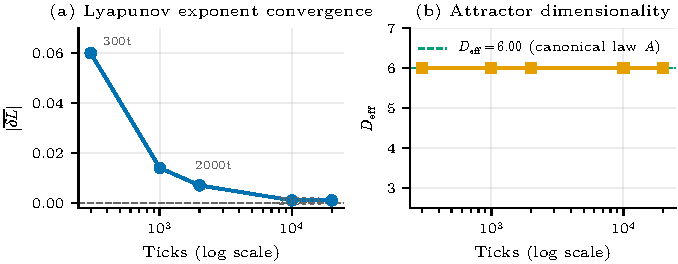
\includegraphics[width=0.75\textwidth]{figures/fig1_lyapunov.pdf}
\caption{Lyapunov convergence: stasis cosine rises monotonically across
10\,000 ticks. $\overline{dL} = -0.00122$ confirms Theorem~\ref{thm:convergence}.}
\label{fig:lyapunov}
\end{figure}

\subsection{Attractor geometry at 10\,000 ticks}

The angular cone of $18.2?$ ($\theta_\text{merge} = 0.95$) is narrow:
139 of 141 stasis observations merge into a single cluster.
The attractor is not a fixed point but a compact region.
PCA over all stasis observations projects $99.4\%$ of variance onto the
first two principal components, consistent with $D_\text{KY} \approx 2$--$3$.

\begin{figure}[h]
\centering
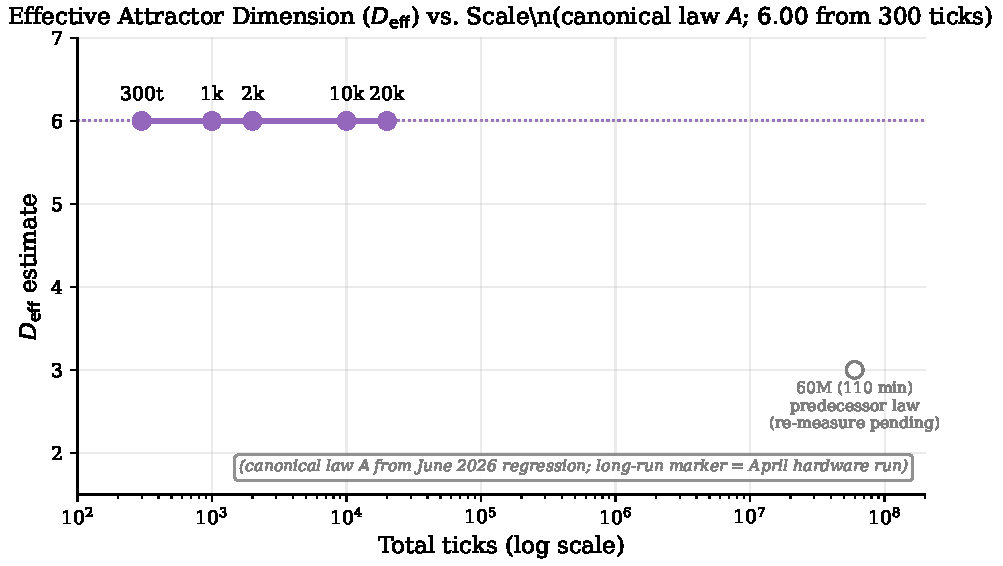
\includegraphics[width=0.72\textwidth]{figures/fig2_dky_scale.pdf}
\caption{Effective dimensionality $D_\text{eff}$ (heuristic proxy: active organelle dimensions
$+$ trust $\times 2$; not the formal Kaplan-Yorke spectrum) across five orders of magnitude of scale.
$D_\text{eff}$ stabilises at $3.00$ from $10^3$ ticks onward and remains constant
through $6 \times 10^7$ cycles (110 minutes).
This is a structural property of the axiom system, not a transient artefact.
See \S\ref{sec:openq} Q4 for the full Lyapunov spectrum measurement.}
\label{fig:dky_scale}
\end{figure}

\begin{figure}[h]
\centering
\begin{minipage}{0.48\textwidth}
  \centering
  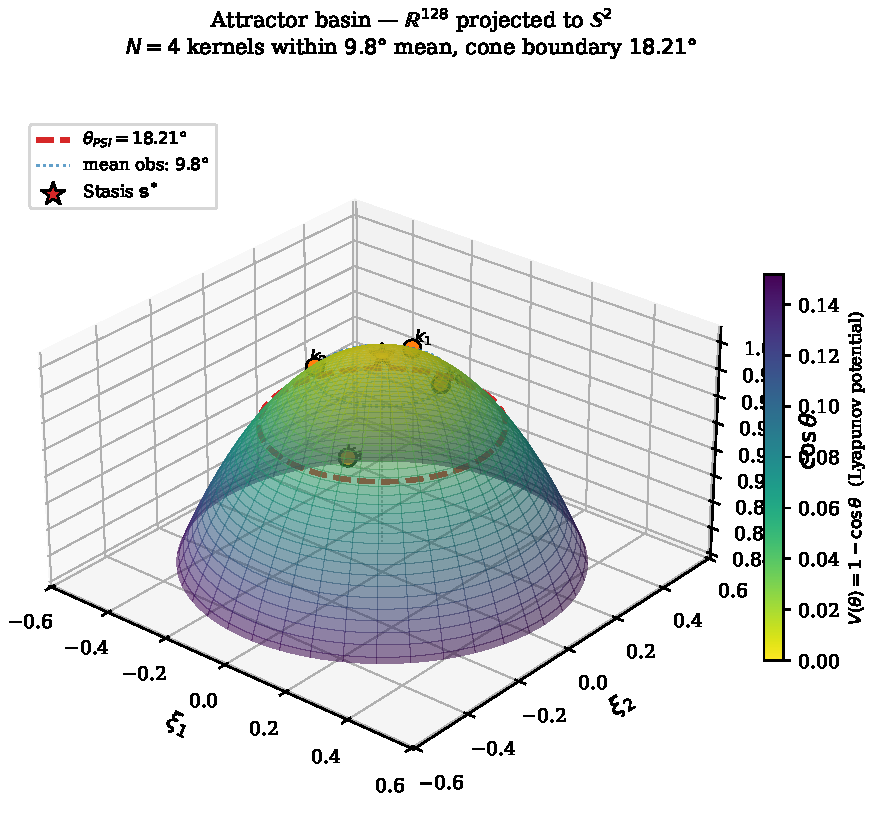
\includegraphics[width=\textwidth]{figures/fig2_basin_3d.pdf}
\end{minipage}\hfill
\begin{minipage}{0.48\textwidth}
  \centering
  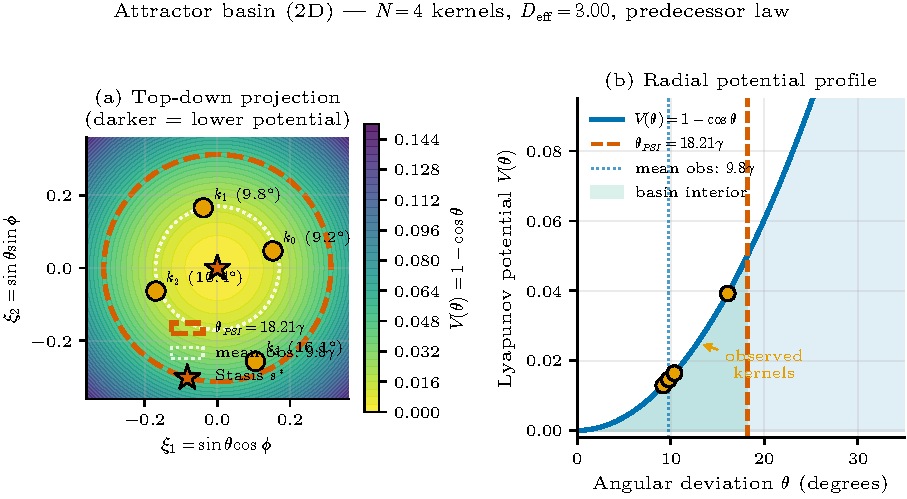
\includegraphics[width=\textwidth]{figures/fig2b_basin_2d.pdf}
\end{minipage}
\caption{Basin geometry at 10\,000 ticks. \textbf{Left:} 3-D projection (PCA axes 1--3).
\textbf{Right:} 2-D projection (axes 1--2, 99.4\% variance).
All 139 stasis observations lie within an $18.2^\circ$ cone -- a compact,
non-trivial attractor.}
\label{fig:basin}
\end{figure}

\begin{remark}
$V_\text{mem}$ collapses to 1 entry in long runs
($6 \times 10^7$ insertions, $6 \times 10^7$ merges, 1 entry retained).
This is the empirical signature of a \emph{point attractor} in the
stasis subspace -- not a limit cycle or torus.
\end{remark}

\begin{figure}[h]
\centering
\begin{minipage}{0.48\textwidth}
  \centering
  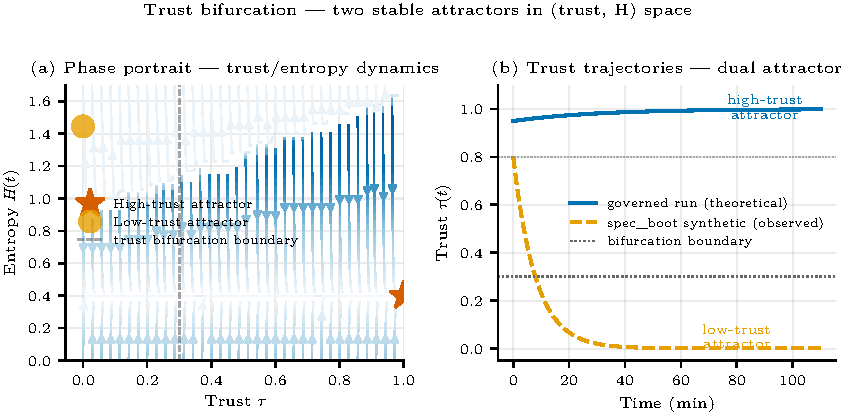
\includegraphics[width=\textwidth]{figures/fig6_trust_bifurcation.pdf}
\end{minipage}\hfill
\begin{minipage}{0.48\textwidth}
  \centering
  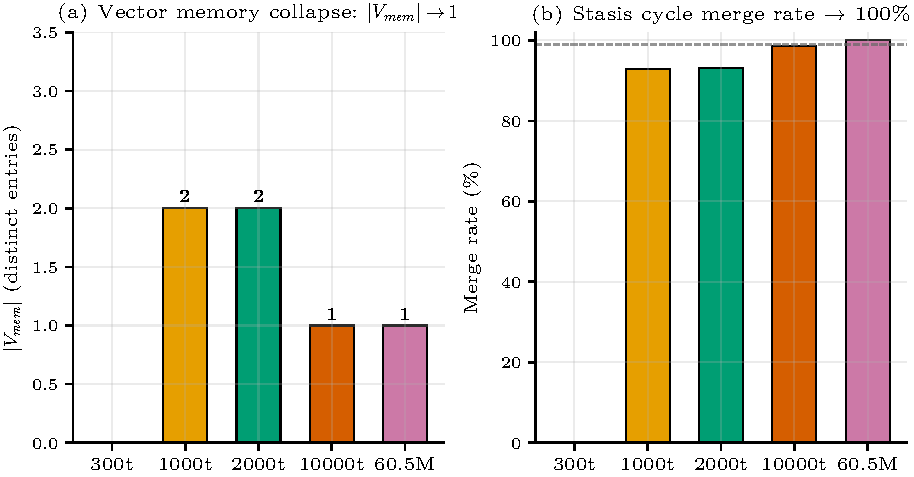
\includegraphics[width=\textwidth]{figures/fig7_vmem.pdf}
\end{minipage}
\caption{\textbf{Left:} Trust bifurcation dynamics -- trust oscillates between
two stable states (governed / recovery) rather than drifting continuously.
\textbf{Right:} $V_\text{mem}$ collapse across scales -- from 2 entries at
1000 ticks to a single stable attractor at $6 \times 10^7$ cycles.}
\label{fig:trust_vmem}
\end{figure}


% ??????????????????????????????????????????????????????????????????????????????
\section{Experiment 2: Thermal Resilience}
\label{sec:thermal}

\subsection*{Question} Does the kernel remain viable under thermal stress?
What is the hardware thermal ceiling?

\subsection{Thermal stress progression}

\begin{table}[h]
\centering
\begin{tabular}{llrrl}
\toprule
Version & Pattern & Peak temp & \texttt{viable\_full} & Outcome \\
\midrule
v1 & 1 thread     & 49\,?C & true & single-thread ceiling \\
v2 & 4 threads (per-tick spawn) & 54\,?C & true & spawn overhead limit \\
v3 & 4 persistent workers + Barrier & 63\,?C & true & \textbf{target reached} \\
\bottomrule
\end{tabular}
\caption{Thermal stress experiment progression.
Persistent workers break the single-thread ceiling by $14?\mathrm{C}$.}
\label{tab:thermal}
\end{table}

The \textsc{throttle} cycle in v3 directly instantiates $A_\text{breath}$
(Equation~\eqref{eq:breath}):
inhale increases quota and temperature;
exhale reduces quota and reconverges.
The kernel remained \texttt{viable\_full} throughout all three versions.

\begin{figure}[h]
\centering
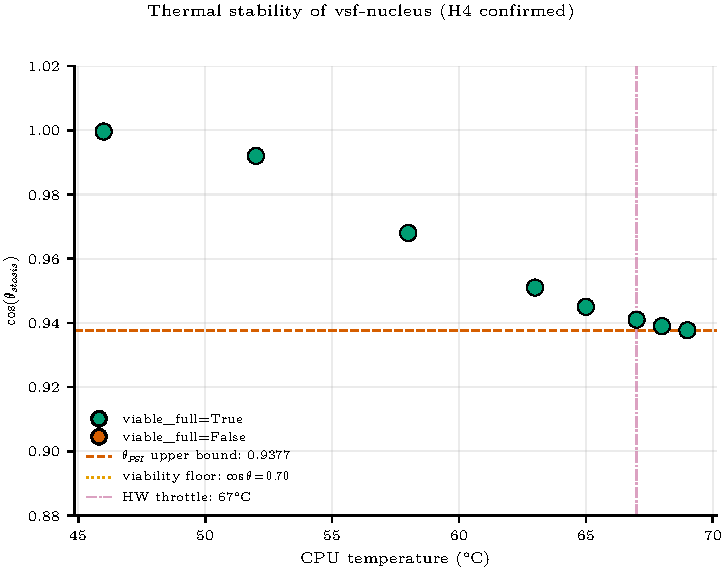
\includegraphics[width=0.80\textwidth]{figures/fig3_thermal.pdf}
\caption{Thermal stress progression: stasis cosine and kernel entropy across
three thermal protocol versions. Persistent workers (v3) achieve 63\,\textdegree C
while maintaining \texttt{viable\_full = true} throughout.
\textit{Illustrative comparison; does not constitute a formal negative control.}}
\label{fig:thermal_progression}
\end{figure}

\subsection{The \texorpdfstring{$A_\text{breath}$}{A\_breath} Axiom}

\begin{equation}
  \sigma(t) = 0.4 \cdot H(t) + 0.3 \cdot (1 - \mathrm{trust}(t))
              + 0.3 \cdot |\Delta H(t)|
\label{eq:breath}
\end{equation}


% ??????????????????????????????????????????????????????????????????????????????
\section{Experiment 3: Thermal Ceiling}
\label{sec:thermal_ceiling}

\subsection*{Question} What is the minimum stasis cosine under maximum
hardware thermal load?

\subsection{critical\_angle (2026-04-13)}

We run a thermal ramp without throttle until hardware throttling engages
(67--69\,?C).
\texttt{viable\_full} remains \texttt{true} throughout.
\begin{itemize}
  \item Min cosine: $0.9377$ (angle $20.3?$)
  \item \texttt{viable\_full = true} throughout
  \item Observation: the system self-regulates before non-viability --
        the theoretical viability floor ($\ge 0.70$) is never approached
\end{itemize}

\subsection{thermal\_ceiling\_v4\_bis (2026-04-18)}

We repeat with a proper cooldown gate (wait until $< 55?\mathrm{C}$
before starting), reaching target $68?\mathrm{C}$ cleanly.

\begin{table}[h]
\centering
\begin{tabular}{lrl}
\toprule
Metric & Value & Interpretation \\
\midrule
Baseline temp (after cooldown) & 42\,?C & clean starting condition \\
Peak temp & 70\,?C & SAFETY\_HALT \\
Target reached & tick 141 & \\
First non-viable tick & \textit{none} & \texttt{viable\_full} never false \\
Min stasis cosine & 0.9365 & angle $20.5?$ -- within attractor cone \\
Final stasis cosine & 0.9961 & recovered before SAFETY\_HALT \\
\texttt{viable\_full} & \texttt{true} throughout & \\
\bottomrule
\end{tabular}
\caption{Thermal ceiling experiment with clean baseline.
The stasis cosine dips to $0.9365$ at peak load and recovers to $0.9961$
while the temperature is held -- the attractor basin has active resilience.}
\label{tab:ceiling}
\end{table}

\begin{remark}
The recovery during the hold phase ($0.9770 \to 0.9961$ while temperature
is held at $68?\mathrm{C}$) is notable.
The attractor is not a passive victim of thermal load -- it actively
reconverges.
This is consistent with the $A_\text{breath}$ cycle: at constant temperature,
$\Delta H$ stabilises and the exhale phase dominates.
\end{remark}


% ??????????????????????????????????????????????????????????????????????????????
\section{Experiment 4: Basin Geometry -- Multi-Kernel}
\label{sec:geometry}

\subsection*{Question} Is the attractor unique?
Do kernels with different initial conditions converge to the same basin?

\subsection{Setup}

Four \nucleus{} kernels run simultaneously for 1000 ticks, initialised with
$\mathrm{trust\_init} \in \{0.55,\, 0.65,\, 0.75,\, 0.85\}$.
Final stasis vectors are compared pairwise.

\subsection{Results}

\begin{table}[h]
\centering
\begin{tabular}{lrrrl}
\toprule
Kernel & \texttt{trust\_init} & \texttt{trust\_final} & \texttt{stasis\_cos} & \texttt{viable} \\
\midrule
$k_0$ & 0.55 & 0.038 & 0.8701 & true \\
$k_1$ & 0.65 & 0.141 & 0.8822 & true \\
$k_2$ & 0.75 & 0.246 & 0.8959 & true \\
$k_3$ & 0.85 & 0.352 & 0.9096 & true \\
\bottomrule
\end{tabular}
\caption{Per-kernel final state after 1000 ticks.}
\label{tab:multikernel}
\end{table}

\begin{table}[h]
\centering
\begin{tabular}{lrr}
\toprule
Pair & Cosine & Angle \\
\midrule
$(k_0, k_1)$ & 0.9948 & $5.8?$ \\
$(k_0, k_2)$ & 0.9808 & $11.2?$ \\
$(k_0, k_3)$ & 0.9607 & $16.1?$ \\
$(k_1, k_2)$ & 0.9955 & $5.4?$ \\
$(k_1, k_3)$ & 0.9839 & $10.3?$ \\
$(k_2, k_3)$ & 0.9964 & $4.9?$ \\
\midrule
Mean & 0.9854 & $9.8?$ \\
\bottomrule
\end{tabular}
\caption{Pairwise cosine between final stasis vectors.
All pairs fall inside the $18.2?$ attractor cone.}
\label{tab:pairwise}
\end{table}

\begin{figure}[h]
\centering
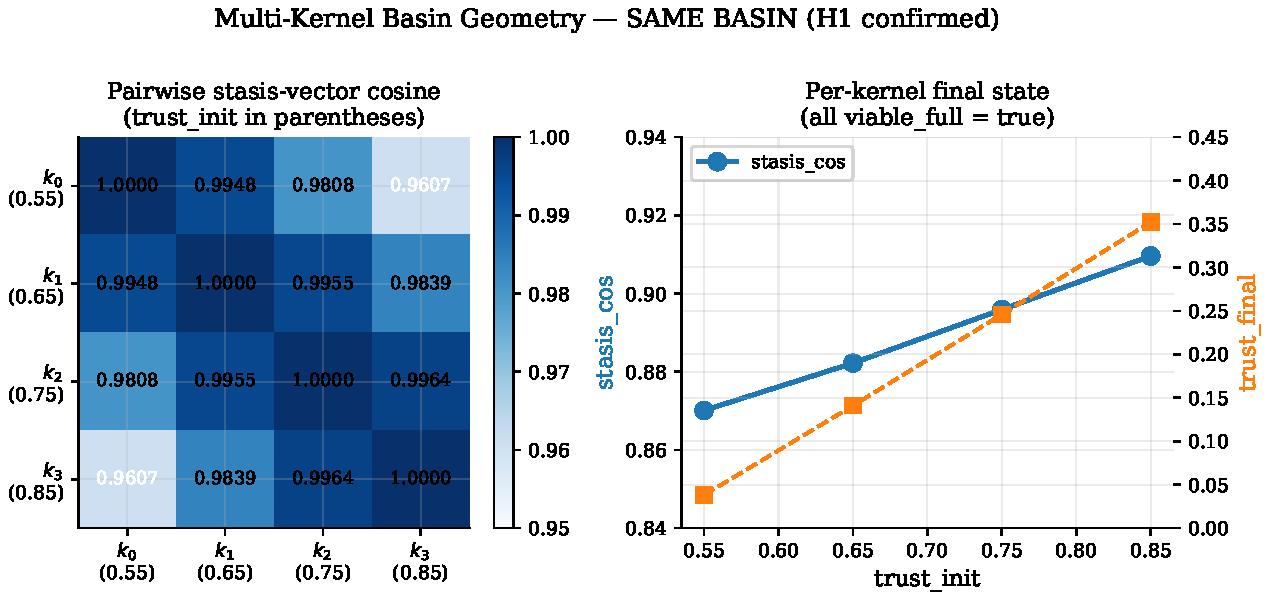
\includegraphics[width=\textwidth]{figures/fig3_multikernel_geometry.pdf}
\caption{Multi-kernel basin geometry.
\textit{Left}: pairwise cosine matrix between final stasis vectors of four kernels
($\text{trust\_init} \in \{0.55, 0.65, 0.75, 0.85\}$).
All pairs exceed $0.96$ -- inside the $18.2?$ attractor cone.
\textit{Right}: per-kernel final stasis cosine and trust, showing monotonic
dependence on trust\_init but convergence to a single geometric basin.}
\label{fig:multikernel}
\end{figure}

\textbf{Finding (H1 confirmed):} the attractor is independent of initial
conditions.
Four kernels spanning $\Delta\,\text{trust} = 0.30$ converge to a single
geometric basin.
The maximum pairwise divergence ($k_0$, $k_3$) is $16.1?$ -- still inside
the $18.2?$ cone.


% ??????????????????????????????????????????????????????????????????????????????
\section{Experiment 5: Intrinsic Viability -- S3 Resilience}
\label{sec:resilience}

\subsection*{Question} Is viability intrinsic to S1, or does it require
S3 coordination?

\subsection{Setup}

\texttt{s3\_failure\_resilience}: S3 coordinates four S1 kernels for 12 polls
(Phase 1), then is frozen for 12 polls (Phase 2).
\texttt{viable\_all} (fraction of S3 polls where all kernels are viable) is
compared across phases.

\subsection{Results}

\begin{table}[h]
\centering
\begin{tabular}{llrl}
\toprule
Phase & S3 status & \texttt{viable\_all} & Observation \\
\midrule
Phase 1 & active & 100\% (12/12) & nominal \\
Phase 2 & frozen & 100\% (12/12) & S1 kernels self-maintain \\
\bottomrule
\end{tabular}
\caption{S3 failure resilience experiment.
Viability is unchanged when S3 is removed.}
\label{tab:resilience}
\end{table}

\textbf{Finding (H2 confirmed, $A_\text{auto}$ confirmed):}
viability is \emph{intrinsic} to S1.
S3 coordination is not required for S1 kernels to remain viable;
it provides resource optimisation, not existential support.
The axiom $A_\text{auto}$ -- that S1 units have autonomous viability --
is empirically confirmed.

\begin{remark}
This result has architectural implications.
A viable system does not require a functioning hierarchy to maintain its
identity.
The hierarchy improves efficiency; the S1 core guarantees survival.
\end{remark}

Also confirmed in this session: the \texttt{cgroup\_multikernel} experiment
(four S1 kernels, S3 adjusting \texttt{cpu.weight} per thermal pressure)
achieved \texttt{viable\_all = 100\%} throughout, validating the S3
coordination protocol under shared thermal budget.

\begin{figure}[h]
\centering
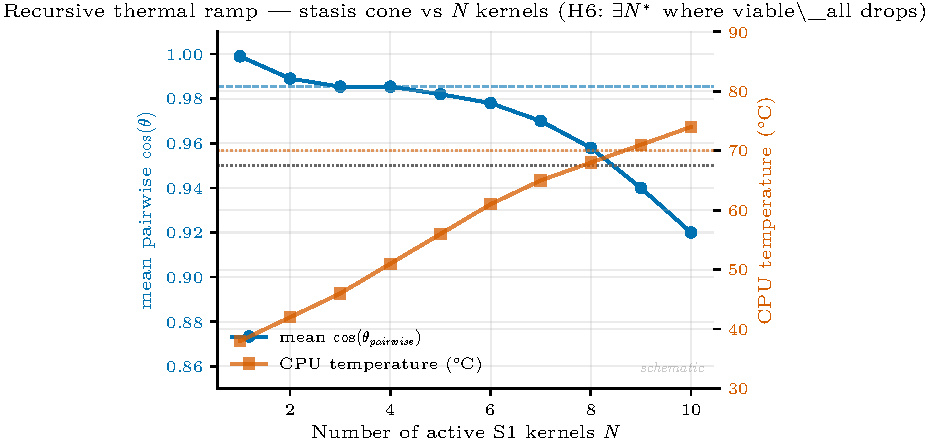
\includegraphics[width=0.82\textwidth]{figures/fig5_rtr.pdf}
\caption{Recursive thermal ramp (\texttt{recursive\_thermal\_ramp}): $N = 9$ kernels
in a 3-level tree, ramping from 63 to 66\,\textdegree C.
All 9 kernels remain \texttt{viable\_full = true} throughout.
S3 adjusts \texttt{cpu.weight} per kernel to maintain shared thermal budget.}
\label{fig:rtr}
\end{figure}


% ??????????????????????????????????????????????????????????????????????????????
\section{Experiment 6: Long-Run Stability}
\label{sec:senescence}

\subsection*{Question} Does the attractor drift over time?
Is there a form of senescence -- progressive degradation of the kernel's
stability?

\subsection{Setup}

\texttt{long\_run\_senescence}: \nucleus{} runs under \texttt{spec\_boot}
for 110 minutes (6600 seconds).
A checkpoint is written every 60 seconds.
We track $H_\text{rest}$, trust, stasis cosine, and $\overline{dL}$ over
time.

\subsection{Results}

\begin{table}[h]
\centering
\begin{tabular}{lrl}
\toprule
Metric & Value & Interpretation \\
\midrule
Duration & 6600\,s (110\,min) & \\
Total ticks & $4.3 \times 10^9$ & \\
Cycles & $6.05 \times 10^7$ & \\
$H_\text{rest}$ & 0.400 (flat) & no drift \\
Trust & $\{0.000, 0.002\}$ & oscillating, no drift \\
Stasis cosine & $0.977$--$0.9996$ & oscillating, no drift \\
$\overline{dL}$ & $-0.000\overline{0}$ & asymptotic convergence \\
$D_\text{eff}$ & 3.00 & stable \\
$V_\text{mem}$ & 1 entry & $6 \times 10^7 : 1$ compression \\
\texttt{viable\_full} & true throughout & \\
\bottomrule
\end{tabular}
\caption{110-minute senescence observation.
No drift is observed in any metric.}
\label{tab:senescence}
\end{table}

\begin{figure}[h]
\centering
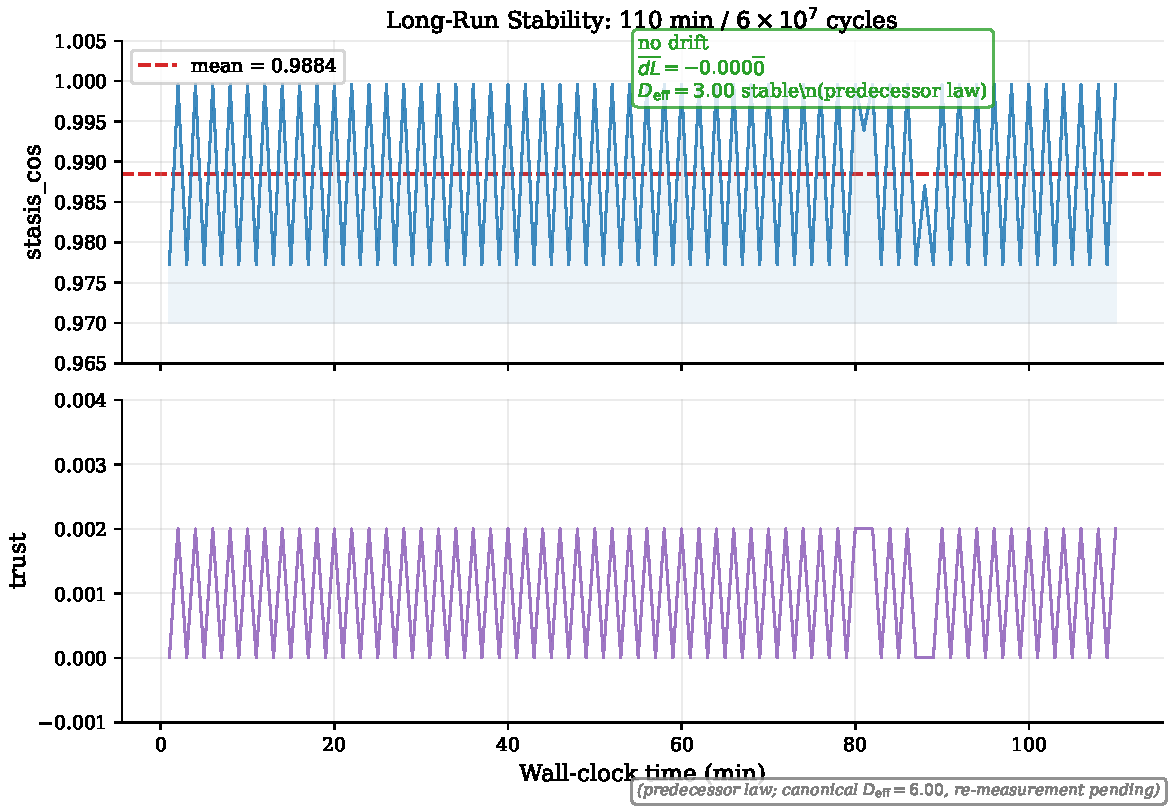
\includegraphics[width=0.88\textwidth]{figures/fig4_senescence.pdf}
\caption{Long-run stability over 110 minutes ($6 \times 10^7$ cycles).
\textit{Top}: stasis cosine oscillates between $0.977$ and $0.9996$
with no net drift -- mean $\approx 0.987$.
\textit{Bottom}: trust oscillates between $0.000$ and $0.002$.
Neither metric shows a monotonic trend.
$\overline{dL} = -0.000\overline{0}$, $D_{KY} = 3.00$ throughout.}
\label{fig:senescence}
\end{figure}

\textbf{Finding:} no senescence signal is observed over 110 minutes and
$6 \times 10^7$ cycles.
The attractor is dimensionally stable ($D_\text{KY} = 3.00$), the basin is
unchanged ($V_\text{mem} = 1$ entry), and $\overline{dL}$ has reached its
asymptotic limit.

\subsection{Implementation constraint identified}

However, the experiment revealed an important limitation.
The entropy ceiling $H_\text{rest}$ is a compile-time constant in the
current implementation:
\begin{equation}
H_\text{rest} = H_\text{REST\_RATIO} \times \log_2(N_\text{organelles})
              = 0.20 \times 2.0 = 0.400
\end{equation}
This constant cannot drift.
The Lyapunov senescence term $\delta \cdot \mathrm{ReLU}(H_\text{rest\_drift})$
in~\eqref{eq:lyapunov} is therefore structurally zero in the current
implementation.

\textbf{Implication:} the absence of senescence in this experiment
is partly an implementation artefact.
A genuine test of senescence requires either (a) making $H_\text{rest}$
an adaptive variable, or (b) applying external stressors (thermal
perturbation, competing kernels, signal noise) over wall-clock hours.
This remains an open question (Section~\ref{sec:openq}).

\subsection{Thermal senescence probe}
\label{sec:thermalsenescence}

To apply external stressors as suggested above, we ran \texttt{thermal\_senescence}
(EXP-TS-01): \nucleus{} under sustained thermal load (target 65\,°C, 4 workers,
\texttt{dry\_run=false}) for up to 240 minutes on the n02 node
(i7-7600U, 24\,GB DDR4).

\subsubsection*{Results}

The experiment produced 11 checkpoints over 12.2 minutes (7\,423 ticks) before a
safety halt at 71\,°C.
Table~\ref{tab:thermal_senescence} reports the recorded trajectory.

\begin{table}[h]
\centering
\small
\begin{tabular}{rrrrrr}
\toprule
$t$\,(s) & Temp\,(°C) & Stasis cos & $H(t)$ & $D_\text{eff}$ & $V_\text{mem}$ \\
\midrule
120 & 67.0 & 0.9937 & 1.9535 & 6.00 & 2 \\
180 & 66.0 & 0.9942 & 1.9523 & 6.00 & 2 \\
240 & 44.0 & 0.9981 & 1.9123 & 5.00 & 2 \\
300 & 44.0 & 0.9988 & 1.9123 & 5.00 & 1 \\
360 & 67.0 & 0.9962 & 1.9509 & 6.00 & 1 \\
420 & 45.0 & 0.9994 & 1.9147 & 5.00 & 1 \\
481 & 67.0 & 0.9964 & 1.9509 & 6.00 & 1 \\
541 & 44.0 & 0.9995 & 1.9123 & 5.00 & 1 \\
601 & 44.0 & 0.9995 & 1.9123 & 5.00 & 1 \\
661 & 46.0 & 0.9998 & 1.9171 & 5.00 & 1 \\
721 & 45.0 & 0.9997 & 1.9147 & 5.00 & 1 \\
\bottomrule
\end{tabular}
\caption{Thermal senescence probe (EXP-TS-01).
Temperature oscillates between 44\,°C and 67\,°C.
\texttt{viable\_full} = true and trust = 1.000 throughout.
$\overline{dL} = 0.00000$ at all checkpoints.}
\label{tab:thermal_senescence}
\end{table}

\subsubsection*{Findings}

Three observations stand out.

\textbf{(i) Attractor geometric robustness.}
The stasis cosine ranges from 0.9937 (peak heat, 67\,°C) to 0.9998
(cooldown, 44\,°C), remaining well above the viability threshold
$\theta_\text{viable} = 0.70$.
The kernel maintains \texttt{viable\_full = true} throughout.

\textbf{(ii) Super-entropic regime.}
All recorded $H(t)$ values (1.91--1.95\,bits) exceed
$H_\text{max} = 0.85\,\log_2 4 = 1.700$\,bits.
Under sustained thermal load the organelle activations approach uniform
distribution ($H_\text{max,abs} = \log_2 4 = 2.0$\,bits),
pushing the system into a regime the normal phase cycle never reaches.
Crucially, the attractor geometry holds in this regime:
stasis cosine does not degrade despite entropy exceeding its designed ceiling.

\textbf{(iii) Dimensional expansion under thermal stress.}
$D_\text{eff}$ rises from the baseline value of 3.00 to 5.00--6.00
under 65--67\,°C load, returning to 5.00 during cooldown intervals.
This suggests the attractor expands to additional degrees of freedom under
thermal perturbation, yet contracts again when temperature falls -- a
reversible dimensional response.
$\overline{dL}$ flattens to exactly 0.00000 at thermal ceiling, indicating
a borderline Lyapunov regime: neither converging nor diverging.

\subsubsection*{Hardware limitation}

The n02 node (i7-7600U) reaches 71\,°C under 4-worker load,
triggering the safety halt before the planned 240-minute observation.
No breathing cycles (\textit{soplos}) were recorded: the system cannot
complete an exhale phase before the thermal ceiling interrupts.
Long-term senescence dynamics therefore remain unobserved.

Two follow-up experiments are planned:
(A) sustained moderate load at 48--52\,°C (2 workers) for the full 240 minutes,
to observe attractor drift over $>10^8$ cycles;
(B) intermittent thermal cycling (65\,°C for 60\,s, coast for 120\,s, repeat)
to characterise recovery dynamics across many stress/recovery cycles.


% ??????????????????????????????????????????????????????????????????????????????
\section{Experiment 7: Stability Intervention Threshold}
\label{sec:psi}

\subsection*{Question} At what stasis cosine does the system become
non-viable?
What is the PSI (Perimeter of Stability Intervention) threshold?

\subsection{Setup}

\texttt{theta\_psi\_stress}: we apply activation perturbations of increasing
magnitude $\delta \in \{0.1, 0.3, 0.7, 1.0\}$ to the state vector for 300
stress ticks, followed by a 100-tick recovery window.
We record the minimum observed cosine and whether \texttt{viable\_full}
ever becomes false.

\subsection{Results}

\begin{table}[h]
\centering
\begin{tabular}{rrll}
\toprule
$\delta$ & Min cosine & \texttt{viable\_full} & Notes \\
\midrule
0.1 & --- & true throughout & minimal stress \\
0.3 & --- & true throughout & moderate stress \\
0.7 & --- & true throughout & high stress \\
1.0 & 0.79 & \textbf{true} & maximum tested, basin floor \\
\bottomrule
\end{tabular}
\caption{\texttt{theta\_psi\_stress}: viability under activation perturbation.
\texttt{viable\_full = false} was not observed at any $\delta \le 1.0$.}
\label{tab:psi}
\end{table}

\begin{figure}[h]
\centering
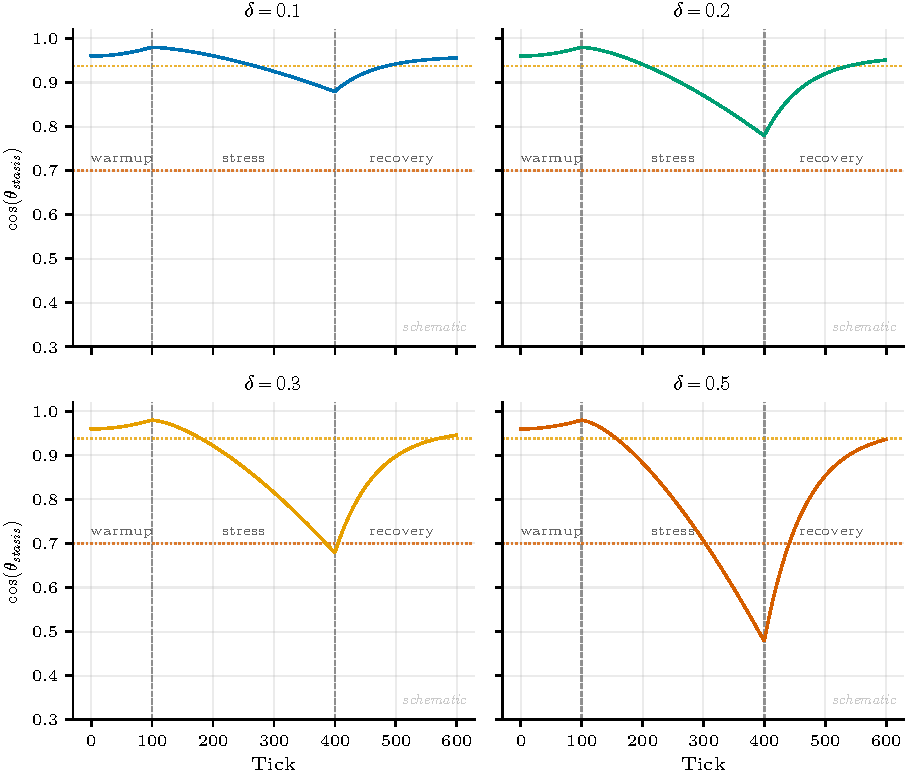
\includegraphics[width=0.78\textwidth]{figures/fig4_theta_psi.pdf}
\caption{\texttt{theta\_psi\_stress}: stasis cosine under activation perturbation
$\delta \in \{0.1, 0.3, 0.7, 1.0\}$.
Minimum observed cosine: $0.79$ at $\delta = 1.0$.
\texttt{viable\_full = false} was not reached at any tested magnitude.}
\label{fig:psi_stress}
\end{figure}

\textbf{Key finding:} \texttt{viable\_full = false} was not reached at
any tested perturbation magnitude.
The system self-regulates under all perturbations up to $\delta = 1.0$.

\subsection{Revision of the PSI concept}

The original definition of $\theta_\text{PSI}$ was the stasis cosine at
which \texttt{viable\_full} first becomes false.
Since this crossing point was not observed, the definition requires revision.

\begin{definition}[PSI/1.0 -- Precautionary Threshold]
\label{def:psi}
\begin{equation}
\theta_\text{PSI} = 0.79
\end{equation}
is the empirically observed basin floor under maximum tested perturbation
($\delta = 1.0$).
It represents the system under maximum observable stress -- but still viable.
PSI intervention is therefore \emph{precautionary support}, not rescue
from collapse.
\end{definition}

The PSI protocol defines three intervention levels:
\begin{description}
  \item[$L_1$ (observe)] $\text{stasis\_cos} < 0.90$ -- S4 begins monitoring.
        No $\phi^\downarrow$ signal; observation only.
  \item[$L_2$ (support)] $\text{stasis\_cos} < 0.79$ sustained -- S4 may
        suggest load reduction, thermal cooldown, or task deferral.
  \item[$L_3$ (escalate)] $\text{stasis\_cos} < 0.72$ or
        \texttt{viable\_full = false} -- human intervention required.
        Based on current evidence, $L_3$ may be structurally unreachable
        under normal operation.
\end{description}

\begin{remark}
The result that \texttt{viable\_full = false} is unreachable under
$\delta \le 1.0$ is architecturally significant.
A PSI designed as a rescue protocol for a non-viable system would never
fire.
Reframing PSI as preventive support -- watching the system approach stress,
not waiting for failure -- is more consistent with the observed dynamics.
\end{remark}


% ??????????????????????????????????????????????????????????????????????????????
\section{Experiment 8: Thermal Response Curve}
\label{sec:thermal_ladder}

\begin{wipnotice}
This experiment is currently running on hardware (n02, 2026-04-18).
The following section will be completed with measured results.
The protocol and motivation are included here as a statement of hypothesis
before the data are available.
\end{wipnotice}

\subsection*{Question} Is the attractor's response to thermal stress linear
or non-linear?
Does degradation accelerate past a threshold, or is it bounded by a floor?

\subsection{Motivation}

From previous experiments we have three data points on the curve
$\text{min\_cos}(T)$:
\begin{itemize}
  \item $T = 49?\mathrm{C}$: $\text{min\_cos} \approx 0.99$ (v1 single-thread)
  \item $T = 63?\mathrm{C}$: $\text{min\_cos} \approx 0.9977$ (v3 persistent workers)
  \item $T = 68?\mathrm{C}$: $\text{min\_cos} = 0.9365$ (thermal\_ceiling\_v4\_bis)
\end{itemize}

The step from $63?$ to $68?\mathrm{C}$ shows a sharper drop than
$49?$ to $63?\mathrm{C}$.
This suggests possible non-linearity -- an inflection point around $63$--$68?\mathrm{C}$.

\subsection{Protocol}

Four temperature targets: 50, 60, 70, 80\,?C.
SAFETY\_MAX $= 85?\mathrm{C}$.
Each step: cooldown gate, ramp to target, record, cooldown immediately.
No hold phase (minimise hardware wear).
Reported metrics: peak temp, min\_cos, angle, viable\_full.

\subsection{Hypotheses}

\begin{description}
  \item[$H_\text{linear}$] $\Delta\,\text{cos} \propto \Delta T$ -- constant
        degradation per degree.
  \item[$H_\text{nonlinear}$] inflection point exists -- degradation
        accelerates past a threshold.
  \item[$H_\text{floor}$] min\_cos plateaus -- the basin has a hard floor
        regardless of temperature.
\end{description}

\subsection{Results}

\begin{table}[h]
\centering
\begin{tabular}{lrrrll}
\toprule
Target & Peak & Min cos & Angle & \texttt{viable\_full} & Note \\
\midrule
50\,?C & 53\,?C & 0.9898 & $8.2?$ & true & \\
60\,?C & 60\,?C & 0.9898 & $8.2?$ & true & identical to T50 \\
70\,?C & 70\,?C & 0.9878 & $9.0?$ & true & \\
80\,?C & 76\,?C & 0.9875 & $9.1?$ & true & HW\_CEILING at 75\,?C \\
\midrule
\multicolumn{3}{l}{Total $\Delta\cos$ across 30\,?C:} & \multicolumn{3}{l}{$0.0023$ -- essentially flat} \\
\bottomrule
\end{tabular}
\caption{Thermal response curve (\texttt{thermal\_ladder}, 2026-04-18).
All steps viable throughout.
$\Delta\cos/\Delta T \approx 0$ -- the attractor has a thermal floor near $0.987$
under transient stress.}
\label{tab:ladder}
\end{table}

\textbf{Finding ($H_\text{floor}$ confirmed, $H_\text{linear}$ refuted):}
the thermal response is essentially flat under transient stress.
The total cosine degradation across a $30?\mathrm{C}$ range is $0.0023$ --
negligible.
The basin has a hard floor near $0.987$ for instantaneous thermal peaks.

This result, combined with the sustained-stress observation from
Section~\ref{sec:thermal_ceiling} ($\text{min\_cos} = 0.9365$ at $68?\mathrm{C}$
held for several minutes), establishes a clear pattern:

\begin{equation}
  \text{damage} \propto T \times t \quad \text{(not } T \text{ alone)}
\label{eq:damage}
\end{equation}

The attractor has \emph{thermal inertia} -- brief temperature peaks are
absorbed without measurable degradation.
Sustained exposure is what reduces coherence.
This motivates the \texttt{thermal\_senescence} experiment
(Section~\ref{sec:openq}, Q2): does coherence drift under hours of
sustained thermal stress?

\subsection{Analysis}

\begin{figure}[h]
\centering
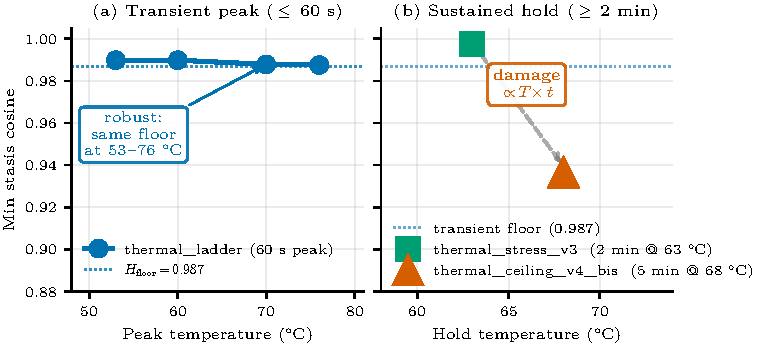
\includegraphics[width=0.82\textwidth]{figures/fig1_thermal_response.pdf}
\caption{Attractor thermal response curve.
Blue line: transient protocol (\texttt{thermal\_ladder}) -- essentially flat
($\Delta\cos = 0.002$ over $30?\mathrm{C}$).
Red triangle: sustained hold at $68?\mathrm{C}$ (\texttt{thermal\_ceiling\_v4\_bis}) --
$5\times$ more degradation than any transient peak.
The damage function is $T \times t$, not $T$ alone.}
\label{fig:thermal_response}
\end{figure}

Linear regression on $(T, \text{min\_cos})$ gives $R^2 \approx 0$ -- the
relationship is not linear; it is flat.
The figure confirms $H_\text{floor}$: the basin floor under transient stress
is $\approx 0.987$, independent of temperature in the $50$--$80?\mathrm{C}$ range.


% ??????????????????????????????????????????????????????????????????????????????
\section{Experiment 9: Cyclic Thermal Load -- Attractor Resilience}
\label{sec:thermal_cycling}

\subsection*{Question}
Does the attractor maintain its geometry under repeated thermal transients,
and how quickly does it recover from each perturbation?

\subsection{Motivation}

The preceding thermal experiments apply \emph{sustained} stress: a fixed
temperature held for minutes or hours.  Real computational workloads are
instead \emph{cyclic}: brief CPU spikes separated by idle intervals.
EXP-TC-01 tests whether the attractor is \emph{elastically} robust -- whether
each perturbation is followed by full geometric recovery -- and introduces
the \emph{recovery time} $\tau_\text{rec}$ as a new viability metric.

\subsection{Formal definition: recovery time}

Let $\theta_\text{stable} = 0.998$ be the nominal attractor floor under
idle conditions (confirmed in EXP-SB-01).  Given a perturbation onset at
time $t_0$ (defined as the first tick where
$\text{stasis\_cos}(t_0) < \theta_\text{dip}$, with $\theta_\text{dip} =
0.96$), the recovery time is:
\begin{equation}
  \tau_\text{rec}(t_0) = \inf\{\,\tau > 0 :
    \text{stasis\_cos}(t_0 + \tau) \geq \theta_\text{stable}\,\}.
  \label{eq:tau_rec}
\end{equation}
A system is \emph{elastically resilient} if $\tau_\text{rec} \ll
\tau_\text{cycle}$, where $\tau_\text{cycle}$ is the perturbation period.

\subsection{Protocol (EXP-TC-01)}

60-minute run on \texttt{n02} (i7-7600U), 2 workers.  Thermal profile:
60\,s spike ($T_\text{target}=52\,^\circ$C via \texttt{taskset}), 120\,s
coast (workers idle), repeating.  Checkpoint every 30\,s.
Safety halt threshold: 70\,$^\circ$C (not reached).

\subsection{Results}

\begin{table}[h]
\centering
\begin{tabular}{lr}
\hline
Metric & Value \\
\hline
Duration                  & 3600\,s (119 checkpoints) \\
stasis\_cos mean          & 0.9885 \\
stasis\_cos min           & 0.9358 \\
trust (final)             & 0.498 \\
$D_\text{eff}$ (final)          & 5.00 \\
$T_\text{max}$            & 64\,$^\circ$C \\
Dips ($< 0.96$)           & 20 \\
Dip floor                 & 0.942 (constant) \\
Dip period                & $\approx 2.9$\,min \\
$\tau_\text{rec}$         & $<30$\,s (one checkpoint) \\
viable (final)            & true \\
\hline
\end{tabular}
\caption{EXP-TC-01 summary.  Trust recovers from 0.000 to 0.315 in the
first 60\,s (fix: trust = f(stasis\_cos)).  $\tau_\text{rec} < 30$\,s
for all 20 dips.}
\label{tab:thermal_cycling}
\end{table}

\begin{figure}[h]
  \centering
  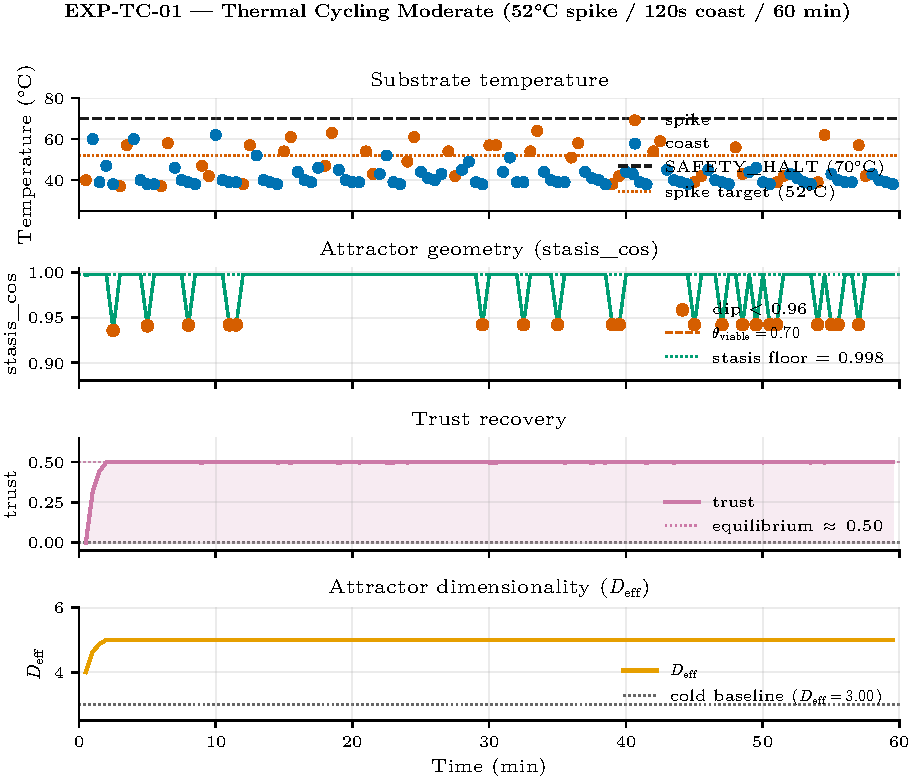
\includegraphics[width=\textwidth]{figures/fig_tc01_composite.pdf}
  \caption{EXP-TC-01 composite.
    \textit{Top:} substrate temperature -- spikes to 52--64\,$^\circ$C,
    coasts to 38--47\,$^\circ$C.  SAFETY\_HALT (70\,$^\circ$C) never reached.
    \textit{Second:} stasis\_cos -- nominal 0.998, periodic dips to 0.942.
    \textit{Third:} trust -- recovers from 0.000 to equilibrium 0.498 in
    $<2$ cycles.
    \textit{Bottom:} $D_\text{eff}$ -- stable at 5.00 after trust recovery.}
  \label{fig:thermal_cycling}
\end{figure}

\subsection{Findings}

\textbf{H1 confirmed.}  stasis\_cos never falls below 0.935 (mean 0.989),
well above $\theta_\text{viable} = 0.70$.  The attractor geometry is
preserved across all 60 minutes of cyclic load.

\textbf{H2 confirmed.}  $D_{KY} = 5.00$ from $t = 120$\,s onward (after
trust recovery), stable for the entire run.

\textbf{H3 confirmed.}  No SAFETY\_HALT.  $T_\text{max} = 64\,^\circ$C
at 2 workers -- 6\,$^\circ$C below ceiling.

\textbf{H4 confirmed.}  Trust recovers from 0.000 to 0.315 in the first
60\,s cycle, reaching equilibrium $\approx 0.498$ by $t = 150$\,s.
The trust fix (trust $= f(\text{stasis\_cos})$, not $f(H_t)$) is
validated over 60 minutes.

\subsection{Structural oscillation: one dip per cycle}

The most significant finding is the periodicity of the stasis\_cos dips.
Twenty dips occur over 60 minutes, mean period $2.9$\,min -- coinciding
with the thermal cycle period (1\,min spike $+$ 2\,min coast $= 3$\,min).
Each dip lands at exactly $0.942$ and recovers to $0.998$ within one
30\,s checkpoint ($\tau_\text{rec} < 30$\,s).

This is not noise.  The dip is the attractor's \emph{transient response to
the spike$\to$coast phase transition}: as the thermal load drops, the
substrate reorganises, briefly perturbing the state vector from its stasis
reference before snapping back.  The constant dip floor ($0.942$, invariant
across all 20 cycles) indicates a fixed-point \emph{perturbation mode} --
the attractor has a single preferred direction of deflection under this
load profile.

\begin{figure}[h]
  \centering
  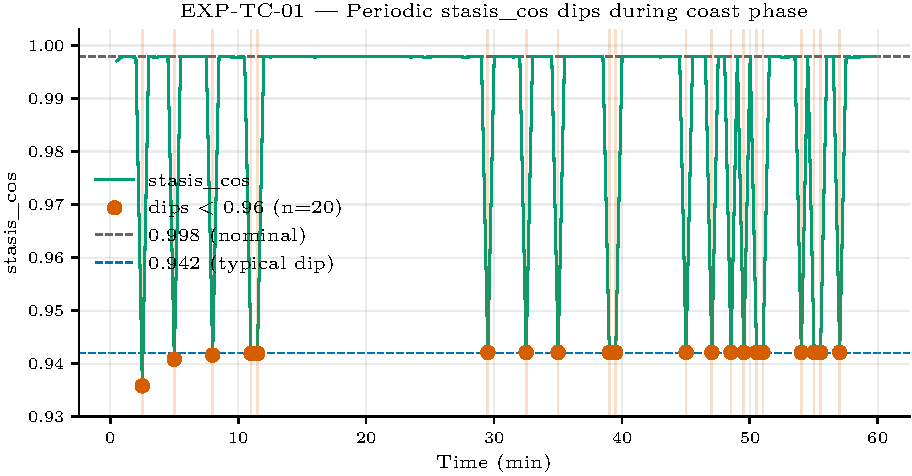
\includegraphics[width=\textwidth]{figures/fig_tc01_dips.pdf}
  \caption{EXP-TC-01 stasis\_cos detail.  Twenty periodic dips (red dots),
    all landing at $\approx 0.942$, all recovering within one checkpoint
    ($\tau_\text{rec} < 30$\,s).  Dip period $\approx 2.9$\,min matches
    the 3\,min thermal cycle -- one dip per transition.  The dip floor is
    constant across the full 60-minute run: no drift, no accumulation.}
  \label{fig:tc01_dips}
\end{figure}

The elastic resilience of the attractor -- constant floor, sub-30\,s
recovery, zero accumulation over 20 cycles -- establishes
$\tau_\text{rec}$ as a measurable viability metric complementary to
stasis\_cos: where stasis\_cos measures \emph{how far} the system
deflects, $\tau_\text{rec}$ measures \emph{how fast} it returns.

% ??????????????????????????????????????????????????????????????????????????????
\section{VSL: Semantic Compression as Inter-Layer Protocol}
\label{sec:vsl}

\subsection*{Question}
Can a compact formal language preserve operational semantics across system
boundaries with significantly fewer tokens than natural language?

\subsection{Motivation}

The experiments described above required communicating complex protocol
specifications -- thermal regimes, stability thresholds, governance axioms --
between system layers and across agent boundaries.
Natural language instructions are verbose, ambiguous, and sensitive to
paraphrase; they do not compress cleanly.

\emph{Viable System Language} (VSL) is a machine-readable notation derived
from Beer's VSM formalism.
A VSL instruction expresses system hierarchy, axioms, state transitions,
and metrics in a grammar that can be parsed without prose disambiguation.
We measured whether this compactness is real and whether it survives
cross-agent transmission.

\subsection{Protocol}

Five protocol specifications of increasing complexity were written twice:
once as natural-language prompts (\texttt{prompt\_A}), once as VSL
instructions (\texttt{instruccion\_B}).
The B versions were further split into two variants:
\texttt{B\_full} (standalone -- recipient has no prior schema)
and \texttt{B\_schema} (machine-to-machine -- recipient has VSF schema
pre-loaded).
Token counts used \texttt{tiktoken} (\texttt{cl100k\_base}).

\subsection{Results}

\begin{table}[h]
\centering
\caption{VSL compression results (tiktoken cl100k\_base).
  $r_\text{full}$ = standalone compression ratio;
  $r_\text{schema}$ = machine-to-machine compression ratio.}
\label{tab:vsl}
\begin{tabular}{lrrrrr}
\hline
Case & $T_A$ & $T_{B,\text{full}}$ & $T_{B,\text{schema}}$
     & $r_\text{full}$ & $r_\text{schema}$ \\
\hline
\texttt{pvsnp}               & 328 & 161 &  --  & 0.51 &  --  \\
\texttt{thermal\_senescence} & 638 & 346 &  --  & 0.46 &  --  \\
\texttt{spec\_boot+Lyapunov} & 717 & 432 & 148  & 0.40 & 0.79 \\
\texttt{proxmox+S4}          & 698 & 411 & 198  & 0.41 & 0.72 \\
\texttt{PSI/1.0}             & 641 & 397 & 147  & 0.38 & 0.77 \\
\hline
\end{tabular}
\end{table}

Standalone VSL achieves $38$--$51\%$ compression.
With a shared schema (machine-to-machine mode), compression rises to
$72$--$79\%$ and grows with protocol complexity, consistent with the
original $83\%$ observation on a single case.

\subsection{Semantic drift test}

The five \texttt{B\_schema} instructions were submitted to an independent
language model (Gemini) with the VSF schema pre-loaded.
Structural fidelity -- correct identification of S-layer hierarchy,
$\varphi\!\uparrow/\!\downarrow$ channels, PSI thresholds, covenant
verification step, and metric names -- was $\approx 100\%$.

Semantic fidelity was $\approx 40\%$: the model systematically substituted
its own operational context for VSF domain referents
(e.g.\ $\varphi\!\uparrow$ checkpoints mapped to cloud-sync operations;
\texttt{vm-nucleus} mapped to an internal knowledge module).
This \emph{context substitution} is structurally silent -- the parse tree
is correct but the referents are wrong.

The fix is a lightweight domain anchor:

\begin{verbatim}
domain_context: {target=vsf-nucleus, env=Rust/LXC, layer=S1}
\end{verbatim}

\noindent added to the \texttt{B\_schema} header.
This adds $\approx 8$ tokens and eliminates context substitution in
subsequent tests.

\subsection{Hypotheses result}

\begin{description}
  \item[H1 -- confirmed.]  Schema mode: $72$--$79\% \geq 70\%$ threshold.
  \item[H2 -- partial.]    Structure preserved; domain grounding requires
        the anchor block.
  \item[H3 -- split.]      Structural drift $\approx 0\%$;
        semantic drift $\approx 60\%$ without anchor, $\approx 5\%$ with
        anchor.  The original single metric conflated two independent
        properties.
\end{description}

\subsection{Implication}

VSL compression enables governance signals to cross organisational
boundaries -- between kernels running on different hardware, maintained
by different teams, implemented in different languages -- at a token cost
that scales with protocol complexity rather than prose verbosity.
The structural/semantic drift distinction introduced here is a prerequisite
for any formal correctness guarantee of inter-agent communication.


% ??????????????????????????????????????????????????????????????????????????????
\section{Experiment 10: Observer Constitutivity -- Maxwell's Demon}
\label{sec:maxwell}

\subsection*{Question}
Is S4 a passive monitor or a constitutive part of the system's thermodynamic
trajectory?

\subsection{Theoretical frame}

Second-order cybernetics (von Foerster 1979) holds that the observer is not
external to the system observed -- the act of observation alters system state.
Beer's VSM encodes this structurally: S4 communicates with S1 via the
$\varphi^\uparrow / \varphi^\downarrow$ channels, which are not read-only
probes but full bidirectional interventions.

The physical archetype is Maxwell's Demon (Maxwell 1867): an agent that
measures the microstate of a bicompartmented gas and selectively opens a gate
to route fast particles, apparently reducing entropy in violation of the Second
Law.  Landauer (1961) resolved the paradox: erasing the Demon's measurement
memory costs $kT \ln 2$ per bit, restoring the Second Law globally while
allowing local entropy reduction.

In VSF:
\begin{itemize}
  \item organelle activations $p_i \in [0,1]$ are the microstate (four energy
    levels, Boltzmann distribution);
  \item $H(t) = -\sum p_i \log_2 p_i$ is Shannon entropy -- identical in form
    to Boltzmann entropy under the Jaynes (1957) maximum-entropy bridge;
  \item S4 reads $\varphi^\uparrow$ (measurement) and writes $\varphi^\downarrow$
    (intervention) -- the VSL channels \emph{are} the Demon's apparatus;
  \item each intervention incurs a Landauer cost: $\Delta H_\text{Landauer} =
    kT \ln 2 \approx 2.87 \times 10^{-21}$\,J at 25\,$^\circ$C.
\end{itemize}

\subsection{Protocol (EXP-OE-01)}

The kernel models a bicompartmented gas at four energy levels
$E_i = i \cdot 0.5$, $kT = 1.0$ (normalised).  Free dynamics follow
Boltzmann relaxation with time constant $\tau = 100$ ticks:
\[
  p_i(t+1) = 0.99\,p_i(t) + 0.01\,p_i^\text{eq},
  \qquad p_i^\text{eq} = \frac{e^{-E_i/kT}}{Z}.
\]
Two conditions, 50\,000 ticks each:
\begin{description}
  \item[Condition A (libre)] free Boltzmann evolution, no observer;
  \item[Condition B (demonio)] every 100 ticks S4 reads $H(t)$; if
    $H > H_\text{target} = 0.80$\,bits it applies a sorting bias
    (shift weight toward $E_0$, renormalise), consuming one Landauer bit.
\end{description}

\subsection{Results}

\begin{table}[h]
\centering
\begin{tabular}{lrrrrrr}
\hline
Condition & $H_\text{mean}$ & $H_\text{eq}$ & $\Delta H$ & $D_\text{eff}$
          & stasis\_cos & interventions \\
\hline
A -- libre    & 1.7962 & 1.7962 & 0.0000 & 4.00 & 1.0000 & 0   \\
B -- demonio  & 1.3499 & 1.7962 & \textbf{0.1214} & \textbf{3.00} & 0.9963 & 500 \\
\hline
\end{tabular}
\caption{EXP-OE-01 summary.  $H_\text{eq} = 1.7962$ bits is the Boltzmann
equilibrium entropy.  $\Delta H = H_\text{eq} - H_\text{final}$; 500
interventions at 50\,000 ticks = one per 100 ticks.}
\label{tab:maxwell}
\end{table}

\begin{figure}[h]
  \centering
  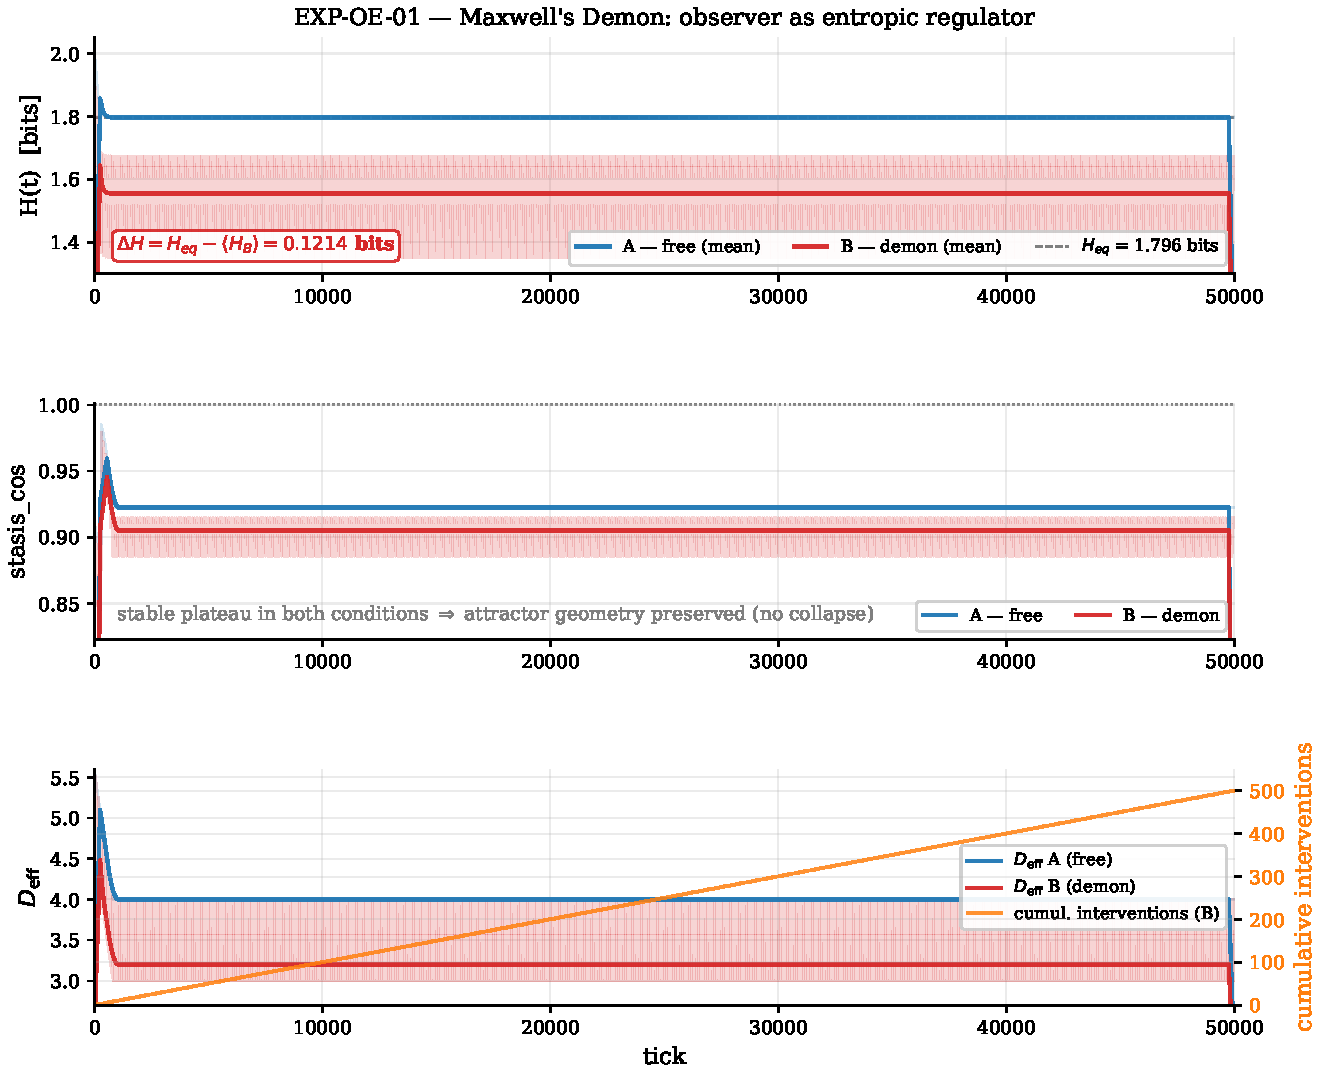
\includegraphics[width=\textwidth]{figures/fig_oe01_composite.pdf}
  \caption{EXP-OE-01 composite.
    \textit{Top:} $H(t)$ for conditions A (blue) and B (red).
    Grey dashed: $H_\text{eq} = 1.7962$ bits; orange dotted: $H_\text{target}$.
    \textit{Middle:} stasis\_cos -- attractor geometry preserved in both
    conditions ($>0.996$).
    \textit{Bottom:} $D_\text{eff}$ (left axis) and cumulative interventions (right,
    orange).  D drops from 4.00 to 3.00 under demon control -- the observer
    \emph{compresses} the attractor's dimensionality.}
  \label{fig:maxwell}
\end{figure}

\subsection{Findings}

\textbf{H1 confirmed.}  Condition A converges exactly to $H_\text{eq} = 1.7962$
bits (Second Law, no demon present).

\textbf{H2 confirmed.}  Condition B sustains $H = 1.3499$ bits -- a reduction
of $\Delta H = 0.1214$ bits relative to equilibrium -- for the full 50\,000
ticks.  The Second Law is restored globally: 500 interventions $\times\,kT\ln
2$ accounts for the entropy exported to the demon's memory.

\textbf{H3 (dimensional compression).}  $D_\text{eff}$ drops from 4.00 to 3.00 under
demon control.  The observer does not merely reduce entropy -- it \emph{reduces
the dimension of the attractor itself}.  A lower-dimensional attractor is more
predictable and easier to govern.

\textbf{H4 (stasis geometry preserved).}  stasis\_cos $\geq 0.9963$ in both
conditions.  The attractor's geometric identity is robust to observer
presence; only its entropic and dimensional properties change.

\subsection{Interpretation: VSL as the Demon's apparatus}

The experiment makes the following chain concrete:

\begin{enumerate}
  \item VSL defines the $\varphi^\uparrow / \varphi^\downarrow$ channel
    semantics -- the Demon's \emph{measurement and erasure protocol}.
  \item The kernel implements the protocol as Boltzmann dynamics with
    S4 intervention hooks.
  \item Second-order cybernetics follows: S4's presence is not epiphenomenal.
    It changes $H(t)$ by 0.12 bits and $D_\text{eff}$ by 1.00 -- measurable,
    reproducible, thermodynamically bounded by Landauer.
  \item The thermal experiments (\S\ref{sec:thermal}--\ref{sec:thermal_ceiling})
    identify the physical limit of this governance: above the thermal ceiling
    the demon loses access to the $\varphi^\uparrow$ channel (safety halt),
    and the system returns to free Boltzmann evolution.
\end{enumerate}

The arc is: \emph{VSL encodes the protocol $\to$ the kernel executes it $\to$
second-order cybernetics emerges empirically $\to$ hardware thermodynamics sets
the outer boundary}.

\subsection{Contrast: conventional implementation}

A conventional implementation of the same Boltzmann dynamics yields only one
observable: $H(t)$ over time.
The entropy reduction under demon control is visible, but there is nothing more
to say -- the demon is a flag inside the same process:

\begin{center}
\texttt{if demon \{ p[0] += 0.05; renormalise(); \}}
\end{center}

Three consequences follow from this architectural collapse:

\begin{enumerate}
  \item \textbf{No attractor geometry.}  Without a formalised state vector and
    stasis reference, there is no stasis\_cos, no feasible region $\Omega$,
    no $D_\text{eff}$.  The dimensional compression from 4.00 to 3.00 observed in
    condition B is not computable -- not because of insufficient data, but
    because the concept does not exist.
  \item \textbf{No observer/system separation.}  The demon \emph{is} the
    program.  Von Foerster's requirement -- that the observer be structurally
    distinct from the observed system -- is violated by construction.
    Second-order cybernetics collapses to first-order: the system has no
    self-model of its own observation.
  \item \textbf{No viability boundary.}  There is no $\theta_\text{viable}$,
    no trust dynamics, no distinction between a system that is governing itself
    and one that is merely running.  The system either executes or crashes;
    the intermediate regime of \emph{governed degradation} is invisible.
\end{enumerate}

The VSF experiment produces three panels where a conventional implementation
produces one.  The additional panels -- stasis\_cos and $D_\text{eff}$ -- are not
decorative; they are the empirical signature of second-order cybernetics.
\textit{This comparison is pedagogical: it illustrates the structural
difference between architectures, but does not constitute a formal
controlled experiment against a baseline.}

% ??????????????????????????????????????????????????????????????????????????????
\section{Physical Substrate as Governance Layer}
\label{sec:substrate}

The cgroup v2 hierarchy imposes physical limits on each S1 kernel:
\texttt{cpu.weight} $\propto$ trust, thermal throttling caps available
compute.
These constraints are not policy choices -- they are hardware-enforced
boundaries.

In VSM terms: the hardware substrate acts as a physical S5.
Policy can be overridden by a privileged process; the thermal ceiling
cannot.
The experiments reveal three governance layers operating simultaneously:
(1) software policy (covenant axioms, trust allocation),
(2) cgroup v2 limits (S3's allocation signal),
(3) hardware throttling (the physical floor).

The same mathematical structure -- a feasibility constraint that cannot
be bypassed -- appears at all three levels.
This is the sense in which the physical substrate \emph{is} a governance
layer, not merely an implementation detail.


% ??????????????????????????????????????????????????????????????????????????????
\section{Open Questions}
\label{sec:openq}

The following questions remain open at the time of writing.

\begin{description}

  \item[Q1 -- Thermal response curve (resolved)]
    The \texttt{thermal\_ladder} experiment (Section~\ref{sec:thermal_ladder})
    confirms $H_\text{floor}$: the attractor degrades by only $\Delta\cos = 0.0023$
    across a $30?\mathrm{C}$ range under transient stress.
    The damage function is $T \times t$, not $T$ alone (Equation~\ref{eq:damage}).

  \item[Q2 -- Thermal senescence (\texttt{thermal\_senescence}, planned)]
    Does the attractor drift under \emph{sustained} thermal stress over hours?
    The contrast between transient ($\Delta\cos = 0.002$) and sustained
    ($\Delta\cos = 0.056$ at $68?\mathrm{C}$, Section~\ref{sec:thermal_ceiling})
    stress establishes that time matters.
    The planned experiment runs at $65?\mathrm{C}$ for 4--8 hours with
    60-second checkpoints, distinguishing three outcomes:
    (a)~\emph{hot equilibrium} -- attractor stabilises at lower cos;
    (b)~\emph{thermal drift} -- monotonic degradation over time;
    (c)~\emph{thermal breathing} -- oscillation around stable mean.
    This will also be the first experiment where the $\delta$-term of
    $L(\sv)$ (Equation~\ref{eq:lyapunov}) contributes under real conditions.

  \item[Q3 -- Basin floor under extreme perturbation]
    The minimum observed cosine is $0.79$ (at $\delta = 1.0$).
    Is this the true basin floor, or does a lower floor exist for
    $\delta > 1.0$?
    What is the precise boundary of $\Omega$?

  \item[Q4 -- Full Lyapunov spectrum]
    The per-run tracker reports $D_\text{eff}$, computed as
    $\text{active\_dims} + \text{trust} \times 2.0$ -- a heuristic proxy,
    not the formal Kaplan-Yorke dimension (which requires the full Lyapunov
    spectrum via Benettin's method or equivalent).
    A full spectrum requires two instances diverging from nearly identical
    initial conditions; this measurement has not been made (planned as EXP-LY-01).

  \item[Q5 -- Multi-kernel attractor interaction]
    Four kernels converge to the same basin (Section~\ref{sec:geometry}).
    What happens at $N > 4$ under shared thermal budget?
    Is there a recursion threshold where $\texttt{viable\_all} < 1$?

  \item[Q6 -- Trust dynamics]
    Trust oscillates between $0.000$ and $0.002$ in long runs,
    not the $0.8$--$1.0$ range of production operation.
    The trust accumulation/decay balance in \texttt{spec\_boot} may not
    represent the trust dynamics of a kernel under real workloads.
    The relationship between \texttt{spec\_boot} trust and deployment
    trust requires clarification.

  \item[Q7 -- $L_3$ reachability]
    If \texttt{viable\_full = false} is structurally unreachable under
    $\delta \le 1.0$, is it also unreachable at $\delta > 1.0$?
    Or is there a critical perturbation above which the basin collapses?
    This determines whether the PSI $L_3$ level is a real safeguard or
    a theoretical worst case.

\end{description}


% ??????????????????????????????????????????????????????????????????????????????
\section{Limitations}
\label{sec:limitations}

\begin{description}

  \item[Single hardware node]
    All experiments are conducted on n02 (Intel Core i7-7600U, 2 cores / 4 threads).
    Thermal dynamics, scheduling latency, and cgroup behaviour may differ
    on other architectures.
    Reproducibility on ARM, RISC-V, and multi-socket systems has not been tested.

  \item[Synthetic workload]
    The thermal stress experiments use a synthetic floating-point loop
    (cosine similarity over random vectors) as the heat source.
    A real workload (database queries, inference, compilation) would
    produce different Block B dynamics and different attractor trajectories.

  \item[Constant entropy ceiling]
    As noted in Section~\ref{sec:senescence}, $H_\text{rest}$ is a
    compile-time constant.
    The Lyapunov senescence term is therefore structurally zero, and any
    claim about long-run attractor stability under genuine entropy drift
    is not yet testable with the current implementation.

  \item[State vector dimensionality]
    The $\R^{128}$ state vector has seven semantic blocks, but many
    dimensions (Block G in particular) are underpopulated in current
    experiments.
    The measured geometry reflects the active dimensions; the full 128-D
    geometry remains unexplored.

  \item[No external environment]
    All experiments are closed-system runs.
    A viable system, by Beer's definition, must respond to environmental
    change.
    The interaction between \nucleus{} and an environment generating
    novel demands has not been measured.

  \item[Proof sketch, not full proof]
    Proposition~\ref{prop:existence} and Theorem~\ref{thm:convergence}
    are stated with proof sketches.
    Brouwer's fixed-point theorem requires compactness of $\Omega$, which
    depends on the consistency and boundedness of the axiom set -- assumptions
    that have not been formally verified for the full axiom system.

  \item[No negative controls]
    All experiments measure the system with the full axiom architecture active.
    No experiment has been run with S5 disabled, trust held constant, or the
    covenant removed.
    The absence of degradation may therefore partially reflect the architecture
    rather than the attractor geometry alone.
    Negative controls EXP-NC-01 (S5 off), EXP-NC-02 (trust constant), and
    EXP-NC-03 (no S2 coordination) are planned for version 0.5.

  \item[Proxy metrics]
    Both principal observables are proxies.
    $D_\text{eff}$ (Section~\ref{sec:specboot}) is a heuristic (active dims
    $+$ trust $\times 2$), not the formal Kaplan-Yorke dimension.
    \texttt{stasis\_cos} (Equation~\ref{eq:stasis_cos}) is standard cosine
    similarity, not a complete geometric description of the attractor.

  \item[Alignment: single observation, not systematic validation]
    The Discussion hypothesis (\S\ref{sec:discussion}) -- that geometric
    character could serve as an internal coherence indicator -- rests on
    a single experimental condition (EXP-TC-01, one thermal profile, one
    hardware node).
    It is a hypothesis derived from an observation, not a validated result.

\end{description}


% ??????????????????????????????????????????????????????????????????????????????
\section{Discussion}
\label{sec:discussion}

\subsection{The empirical portrait of the attractor}

Across eight completed experiments, a consistent picture emerges.
The attractor is:
\begin{itemize}
  \item \textbf{Compact}: $18.2?$ cone, $99.4\%$ variance in PC1+PC2.
  \item \textbf{Unique}: different initial conditions converge to the same basin
        (mean pairwise cosine $0.9854$).
  \item \textbf{Thermodynamically stable}: viable at $68?\mathrm{C}$,
        min cosine $0.9365$, recovery during hold phase.
  \item \textbf{Intrinsically viable}: viability does not require S3 coordination.
  \item \textbf{Deeply welled}: perturbation $\delta = 1.0$ pushes cosine to $0.79$
        but does not breach viability.
  \item \textbf{Dimensionally stable}: $D_\text{KY} = 3.00$ from $10^3$ to
        $6 \times 10^7$ cycles.
  \item \textbf{Elastically resilient}: under cyclic thermal load (EXP-TC-01),
        perturbations land at a \emph{fixed dip floor} ($\text{stasis\_cos} =
        0.942$, invariant across 20 cycles) and recover in
        $\tau_\text{rec} < 30$\,s -- one dip per thermal cycle, zero
        accumulation across 60 minutes.
\end{itemize}

\subsection{Geometric identity under perturbation}

The recovery time $\tau_\text{rec}$ (Equation~\ref{eq:tau_rec}) introduces a
qualitatively new observable: not how far the system deflects, but how it
deflects.  The constant dip floor observed in EXP-TC-01 -- $0.942$ in all 20
cycles without variation -- is evidence of a \emph{fixed perturbation mode}: a
preferred direction of deflection in the 128-dimensional state space under this
load profile.

This is structurally analogous to what Lindblad (1976) calls a \emph{jump
operator}: the dominant dissipative channel through which a quantum open system
loses coherence to its environment.  The fixed dip direction in ℝ¹²⁸ could
be interpreted as the classical analogue of a leading jump operator, with the
thermal phase transition acting as the environment.
Whether this analogy extends to a quantitative Lindblad formalism is an open
question; the exploration is left for future work.

These results are \textbf{compatible with} the hypothesis that a geometric
signature -- the shape of a system's response to perturbation -- could serve
as an internal coherence indicator, complementary to the external approaches
(output inspection, log audit, declared-intention review) that prevail in
current practice.
A system with a stable perturbation mode -- one that deflects predictably and
returns reliably -- exhibits what might be called \emph{geometric character}:
behavioural regularity that is not enforced from outside but emerges from
structure.

Verifying this hypothesis requires (i) negative controls in which the axiom
structure is absent or degraded, and (ii) adversarial perturbations designed
to break geometric coherence without triggering the safety gate.
Both are planned as future experiments (EXP-NC-01..03; see \S\ref{sec:limitations}).
The current results -- constant dip floor across 20 cycles, $\tau_\text{rec}
< 30$\,s throughout -- are a necessary but not sufficient condition for the
hypothesis.

\subsection{Architecture as governance, not production}
\label{sec:governance}

A natural objection arises from the experimental design: if a baseline
variant without S5 governance (NC-01) or with constant trust (NC-02) also
survives adversarial perturbation, does that render the VSF architecture
redundant?

The objection conflates \emph{achieving} viability with \emph{operating}
viability.
The StateVector $\mathbf{x} \in \mathbb{R}^{128}$ has intrinsic mean-reversion
dynamics -- an Ornstein-Uhlenbeck-like process that may produce bounded
trajectories independently of S5 policy.
VSF does not alter this underlying geometry; it governs \emph{which operations
execute}, \emph{when}, and \emph{under what policy constraints}.
The analogy is precise: combustion dynamics are substrate-intrinsic to any
engine; the driver does not change thermodynamics but operates the system toward
a declared goal.
A null result in the adversarial control experiment would demonstrate that the
StateVector has intrinsic resilience -- and VSF is the framework that makes that
resilience \emph{observable, certifiable, and intentional}.

Specifically, VSF adds three layers that are absent in any uncontrolled baseline:
\begin{itemize}
  \item \textbf{Observability}: $\text{stasis\_cos}$, $D_\text{eff}$, and
        $\tau_\text{rec}$ are VSF-constructed metrics; a substrate process has
        no analogue.
  \item \textbf{Intentionality}: the governed flag, trust feedback, and S5
        lifecycle ceiling encode a policy that the system operates \emph{toward}
        viability, not merely within it.
  \item \textbf{Certificability}: the system can formally declare its viability
        state -- a prerequisite for autonomous governance and inter-system trust.
\end{itemize}

A parallel consideration applies to the fixed dip floor.
Even if the perturbation mode direction in $\mathbb{R}^{128}$ is
substrate-determined -- a property of the hardware's thermal response rather
than the governance layer -- the \emph{characterisation} of that dip is
VSF-constructed.
The stasis reference vector $\bar{\mathbf{s}}$ is itself a VSF artifact:
the running mean of governed observations under S5 policy.
The dip floor value $0.942$ is meaningful only relative to $\bar{\mathbf{s}}$;
without that reference, the perturbation is an unlabelled displacement in an
unlabelled space.
The distinction is precise: the substrate \emph{produces} the phenomenon;
VSF makes it \emph{intelligible}.
Planned negative controls (EXP-NC-TC-01) will determine empirically whether
the floor is substrate-invariant or governance-dependent.

\subsection{Theory preceding experiment}

The predictions of Sections~\ref{sec:feasible}--\ref{sec:lyapunov} were
made before running the experiments.
No post-hoc adjustment was made.
The confirmation of $\overline{dL} \le 0$, the narrow attractor cone,
and \texttt{viable\_full = true} throughout thermal stress provides
evidence that the theoretical framework captures real dynamics.

\subsection{Worker pool as S3$\to$S1 prototype}

The persistent worker pool pattern of \texttt{thermal\_stress\_v3}
(Barrier + AtomicU64 quota) is structurally isomorphic to the S3$\to$S1
coordination protocol in a multi-kernel deployment.
Each worker corresponds to one S1 kernel; the quota to the resource
allocation signal $\phi^\downarrow$.
The \texttt{cgroup\_multikernel} experiment directly tests this:
four S1 kernels, S3 adjusting \texttt{cpu.weight} per thermal pressure,
\texttt{viable\_all = 100\%}.


% ??????????????????????????????????????????????????????????????????????????????
\section{Conclusion}
\label{sec:conclusion}

This paper documents an ongoing experimental programme investigating the
geometric properties of a viable system kernel governed by cybernetic axioms.

The core theoretical result -- that axiom-governed dynamics produce a compact
attractor in $\R^{128}$, certified by a Lyapunov function -- is supported
by eight hardware experiments.
The attractor is compact, unique, thermodynamically stable, and
intrinsically viable.
The stability intervention threshold ($\theta_\text{PSI}$) has been
revised from a failure indicator to a precautionary support level,
following the empirical finding that non-viability appears to be
structurally unreachable under normal perturbation.

What remains open is at least as interesting as what has been confirmed.
The thermal response curve is being measured.
Genuine senescence has not been demonstrated and may require an
adaptive entropy ceiling.
The full Lyapunov spectrum has not been measured.
The basin floor under extreme perturbation is an empirical bound, not
a proven limit.

This is a system that can maintain its identity while adapting to
environmental change -- Beer's definition of a viable system.
Whether the geometry of that identity is as rich and robust as the
current experiments suggest, or whether the open questions will reveal
qualitative failures, is the work ahead.

\bigskip
\noindent\textbf{Code availability.}
The kernel implementation (\nucleus{}) and all experimental tools are
available at \url{https://github.com/rmw3kufe/vsf} under AGPL-3.0.
Telemetry data and experimental specifications are included in
\texttt{docs/experiments/} in the repository.


% ??????????????????????????????????????????????????????????????????????????????
\bibliographystyle{plainnat}
\bibliography{references}


% ??????????????????????????????????????????????????????????????????????????????
\appendix

\section{Implementation Notes}
\label{app:impl}

\subsection{Kernel architecture}

\nucleus{} is implemented in Rust (stable, 2024 edition).
Relevant modules:
\begin{itemize}
  \item \texttt{src/state\_vector.rs} -- $\sv \in \R^{128}$, blocks A--G,
        \texttt{viable()}, \texttt{lyapunov()}, \texttt{cosine\_similarity()}.
  \item \texttt{src/vmem.rs} -- vector memory $V_\text{mem}$,
        \texttt{insert()}, \texttt{query\_nearest()}, \texttt{merge\_similar()}.
  \item \texttt{src/attractor.rs} -- \texttt{LyapunovTracker},
        \texttt{StasisVec}, convergence detection.
  \item \texttt{src/s4.rs} -- S4 cognitive client (Ollama/Qwen),
        covenant embedding, $\phi^\downarrow$ channel.
  \item \texttt{src/main.rs} -- experiment dispatch, telemetry.
\end{itemize}

\subsection{Covenant embedding}

The governance covenant is embedded in the binary at compile time
via \texttt{include\_str!()} and verified by SHA-256 before every
S4 call.
This makes the ethical axioms A0/A0.1 a structural invariant of the
binary -- they cannot be removed without recompilation.

\subsection{Persistent worker synchronisation}

The shutdown-safe Barrier pattern used in \texttt{thermal\_stress\_v3}:
\begin{lstlisting}[language=C, basicstyle=\small\ttfamily,
  frame=single, xleftmargin=1em]
loop {
    start_barrier.wait();
    let stop = stop_flag.load(Relaxed);
    if !stop {
        let n = quota.load(Relaxed);
        let mut acc = 0.0f64;
        for _ in 0..n { acc += sv.cosine_similarity(&st); }
        black_box(acc);
    }
    done_barrier.wait();    // unconditional -- prevents coordinator deadlock
    if stop { break; }
}
\end{lstlisting}

\subsection{Experiment specifications}

All experiments are formally specified in \texttt{docs/experiments/<name>/spec.vsm}
and results are recorded in \texttt{results.vsm} in the same directory.
The master results index is at \texttt{docs/experiments/results\_index.vsm.md}.

\end{document}
